\documentclass[a4paper,
fontsize=11pt,
%headings=small,
oneside,
numbers=noperiodatend,
parskip=half-,
bibliography=totoc,
final
]{scrartcl}

\usepackage[babel]{csquotes}
\usepackage{synttree}
\usepackage{graphicx}
\setkeys{Gin}{width=.8\textwidth} %default pics size

\graphicspath{{./plots/}}
\usepackage[ngerman]{babel}
\usepackage[T1]{fontenc}
%\usepackage{amsmath}
\usepackage[utf8x]{inputenc}
\usepackage [hyphens]{url}
\usepackage{booktabs} 
\usepackage[left=2.4cm,right=2.4cm,top=2.3cm,bottom=2cm,includeheadfoot]{geometry}
\usepackage[labelformat=empty]{caption} % option 'labelformat=empty]' to surpress adding "Abbildung 1:" or "Figure 1" before each caption / use parameter '\captionsetup{labelformat=empty}' instead to change this for just one caption
\usepackage{eurosym}
\usepackage{multirow}
\usepackage[ngerman]{varioref}
\setcapindent{1em}
\renewcommand{\labelitemi}{--}
\usepackage{paralist}
\usepackage{pdfpages}
\usepackage{lscape}
\usepackage{float}
\usepackage{acronym}
\usepackage{eurosym}
\usepackage{longtable,lscape}
\usepackage{mathpazo}
\usepackage[normalem]{ulem} %emphasize weiterhin kursiv
\usepackage[flushmargin,ragged]{footmisc} % left align footnote
\usepackage{ccicons} 
\setcapindent{0pt} % no indentation in captions

%%%% fancy LIBREAS URL color 
\usepackage{xcolor}
\definecolor{libreas}{RGB}{112,0,0}

\usepackage{listings}

\urlstyle{same}  % don't use monospace font for urls

\usepackage[fleqn]{amsmath}

%adjust fontsize for part

\usepackage{sectsty}
\partfont{\large}

%Das BibTeX-Zeichen mit \BibTeX setzen:
\def\symbol#1{\char #1\relax}
\def\bsl{{\tt\symbol{'134}}}
\def\BibTeX{{\rm B\kern-.05em{\sc i\kern-.025em b}\kern-.08em
    T\kern-.1667em\lower.7ex\hbox{E}\kern-.125emX}}

\usepackage{fancyhdr}
\fancyhf{}
\pagestyle{fancyplain}
\fancyhead[R]{\thepage}

% make sure bookmarks are created eventough sections are not numbered!
% uncommend if sections are numbered (bookmarks created by default)
\makeatletter
\renewcommand\@seccntformat[1]{}
\makeatother

% typo setup
\clubpenalty = 10000
\widowpenalty = 10000
\displaywidowpenalty = 10000

\usepackage{hyperxmp}
\usepackage[colorlinks, linkcolor=black,citecolor=black, urlcolor=libreas,
breaklinks= true,bookmarks=true,bookmarksopen=true]{hyperref}
\usepackage{breakurl}

%meta
%meta

\fancyhead[L]{L. Freyberg\\ %author
LIBREAS. Library Ideas, 43 (2023). % journal, issue, volume.
\href{https://doi.org/10.18452/...}{\color{black}https://doi.org/10.18452/...}
{}} % doi 
\fancyhead[R]{\thepage} %page number
\fancyfoot[L] {\ccLogo \ccAttribution\ \href{https://creativecommons.org/licenses/by/4.0/}{\color{black}Creative Commons BY 4.0}}  %licence
\fancyfoot[R] {ISSN: 1860-7950}

\title{\LARGE{Erhebung zum Frauenanteil in Leitungspositionen an deutschen Bibliotheken}}% title
\author{Julia Bartlewski} % author

\setcounter{page}{1}

\hypersetup{%
      pdftitle={Erhebung zum Frauenanteil in Leitungspositionen an deutschen Bibliotheken},
     pdfauthor={Julia Bartlewski},
      pdfcopyright={CC BY 4.0 International},
      pdfsubject={LIBREAS. Library Ideas, 43 (2023).},
      pdfkeywords={Frauen, Leitungspositionen, Gläserne Decke, Öffentliche Bibliotheken, Wissenschaftliche Bibliotheken, Verteilung Geschlecht},
      pdflicenseurl={https://creativecommons.org/licenses/by/4.0/},
      pdfurl={https://doi.org/10.18452/27071},
      pdfdoi={10.18452/27071},
      pdflang={de},
      pdfmetalang={de}
     }



\date{}
\begin{document}

\maketitle
\thispagestyle{fancyplain} 

%abstracts
\begin{abstract}
\noindent
\textbf{Kurzfassung}: Geschlechterverhältnisse auf dem Arbeitsmarkt sind Gegenstand zahlreicher Debatten und im Zuge eines sozialen Wandels in das kollektive Bewusstsein gerückt. Der Arbeitsbereich \enquote{Bibliothek} ist ein frauendominiertes Feld mit einem Frauenanteil von über 74\%. Interessanterweise liegen jedoch keine aktuellen umfassenden statistischen Auswertungen über Frauen in Leitungspositionen an deutschen Bibliotheken vor. Vor dem Hintergrund der Leitfrage, wie hoch der Anteil von Frauen in der obersten Hierarchieebene an deutschen Bibliotheken ist, präsentiert der vorliegende Artikel die Ergebnisse einer quantitativen Erhebung. Diese werden in einen theoretischen Kontext eingebettet, in dem Forschungsaspekte aus verschiedenen wissenschaftlichen Disziplinen, wie der Geschlechter- oder Organisationsforschung, vorangestellt werden.

Dieser Beitrag beruht auf einer Masterarbeit aus dem Jahr 2021 am Institut für Bibliotheks- und Informationswissenschaft der Humboldt Universität zu Berlin.

\textbf{Abstract}:Gender proportions in the employment sector are the subject of numerous debates and have moved into the collective awareness as a result of social change. The \enquote{library} work area is a female-dominated field with a share of women of over 74\%. Interestingly, however, there are no current detailed statistical evaluations of women in management positions in German libraries. Against the background of the main question regarding the proportion of women at the top hierarchical level in German libraries, this article presents the results of a quantitative survey. These are embedded in a theoretical context in which research aspects from various scientific disciplines, such as gender or organizational research, are presented.

This article is based on a master's thesis written in 2021 at the Institute of Library and Information Science at the Humboldt Universität zu Berlin.

\begin{center}\rule{0.5\linewidth}{0.5pt}\end{center}
\end{abstract}

%body
\hypertarget{einleitung}{%
\section{1. Einleitung}\label{einleitung}}

Die Teilhabe von Frauen am Erwerbsleben sowie Gleichstellungsthematiken
sind spätestens mit dem Zweiten Führungspositionen-Gesetz (FüPoG II) im
August 2021 wieder deutlich ins gesellschaftliche Bewusstsein gerückt
(BMFSFJ, 2021). Ziel ist, den Anteil von Frauen in Führungspositionen zu
erhöhen. Die Gleichstellung von Frau und Mann im Sinne einer
Nachhaltigkeitspolitik ist ein wichtiges gesamtgesellschaftliches Thema
und die Frage nach der Quote von Frauen in Leitungspositionen an
Bibliotheken ist in diesem Kontext relevant für den
bibliothekswissenschaftlichen Diskurs. Allerdings lag zum Zeitpunkt der
Erstellung dieser Untersuchung im Jahr 2021 keine Auswertung zu dieser
Frage vor. Insbesondere für ein Berufsfeld, das zu den sogenannten
\enquote{Frauenberufen} zählt, ist die fehlende Datenlage ein Desiderat,
das dieser Beitrag in einem ersten Schritt aufarbeitet. Vor dem
Hintergrund der Leitfrage, wie hoch der Anteil von Frauen in der
obersten Hierarchieebene an deutschen Bibliotheken ist, erfolgt eine
quantitative Erhebung anhand von Adressbüchern und Verzeichnissen. Als
Quellen werden dabei die Mitgliederliste des deutschen
Bibliotheksverbands, das Jahrbuch der deutschen Bibliotheken sowie das
Jahrbuch der öffentlichen Bibliotheken herangezogen. Aus der
übergeordneten Leitfrage ergeben sich noch weitere Fragen, die in die
Auswertung mit einbezogen werden. Gibt es Unterschiede in der Verteilung
bei öffentlichen und wissenschaftlichen Bibliotheken? Wie ist das
Verhältnis in verschiedenen Bibliotheksgrößen?

Charakteristisch für die deutsche Bibliothekslandschaft ist deren
Unterscheidung in zwei große Sparten, die der öffentlichen (ÖB) und der
wissenschaftlichen Bibliotheken (WB). Diese \enquote{ausnehmend deutsche
Geschichte der bibliothekarischen Spartentrennung} (HACKER 2002: S. 3)
hat sich seit Beginn des 20. Jahrhunderts manifestiert und
Ausbildungsstrukturen, Verbandsarbeiten und Berufsbilder über Jahre
geprägt. Auch wenn durch unterschiedliche bibliothekspolitische
Bemühungen -- als Beispiele zu nennen sind der \enquote{Bibliotheksplan
`73} sowie das Strukturpapier \enquote{Bibliotheken `93} -- und die
Aufgabe spartenspezifischer Studiengänge Schritte zur Aufhebung der
Spartentrennung unternommen wurden, ist das Unterscheidungsmerkmal in ÖB
und WB weiterhin ein strukturierendes Element im Fachdiskurs (Ebd.: S.
29). Für die Erhebung in diesem Beitrag wurde die Zweiteilung der
Bibliothekslandschaft in ÖB und WB daher beibehalten, da auch die
vorliegenden Quellen dieser folgen.

Die Ungleichstellung von Frauen und Männern auf dem Arbeitsmarkt ist
Untersuchungsgegenstand verschiedener wissenschaftlicher Disziplinen,
wie der Geschlechter- oder Organisationsforschung. Für eine
Kontextualisierung werden vor der Auswertung der Erhebung daher
verschiedene theoretische Konzepte und Definitionen sowie bisherigen
Studien, die sich dezidiert mit dem Thema Frauen in Führungspositionen
an Bibliotheken befassen, kurz vorgestellt und zusammengefasst.

\hypertarget{frauenberuf-bibliothekarin}{%
\section{2. Frauenberuf
Bibliothekar:in}\label{frauenberuf-bibliothekarin}}

Wie eingangs benannt, gehört der Bibliotheksbereich zu den sogenannten
\enquote{Frauenberufen}. Man unterscheidet generell zwischen
Männerberufen, Frauenberufen und Mischberufen. Für ein Verständnis
dieser Bezeichnungen muss man zunächst das Prinzip der beruflichen
Geschlechtersegregation thematisieren, eine Terminologie aus dem Bereich
der Arbeitsmarktforschung. Für die Definition der Termini
\enquote{Frauen- und Männerberuf} ist das Prinzip der horizontalen
Segregation entscheidend. Dies meint \enquote{die ausgeprägte Trennung
von erwerbstätigen Frauen und Männern in unterschiedlichen Berufen}
(HAUSMANN/KLEINERT 2014: S. 1). Demnach wählen Frauen häufiger
Dienstleistungsberufe in Bereichen wie Gesundheitswesen oder Soziales
und Erziehung, wohingegen Männer sich signifikant häufiger für
technische Berufe entscheiden (Ebd.).

Die Unterscheidung zwischen Misch-, Frauen- und Männerberufen erfolgt
anhand des Frauenanteils in einem Beruf. Der vorliegende Beitrag folgt
dabei der Definition, die sich bei Anne Busch-Heizmann findet (2015: S.
572).\footnote{In der Literatur werden teilweise unterschiedliche
  Grenzwerte genannt, jedoch nur mit geringfügigen Abweichungen (ein
  Vergleich dazu findet sich bei BUSCH 2013: S. 117). Ebenfalls folgen
  Hausmann und Kleinert dieser Definition in ihrer Studie von 2014 (S.
  4).} Demnach findet sich in einem Männerberuf ein Frauenanteil von bis
zu 30\%. Bei einem Frauenanteil ab 70\% spricht man von einem
Frauenberuf. Im prozentualen Zwischenbereich liegen die geschlechtlich
gemischten Berufe.

Für die Entwicklung der Zahlen im Bibliothekswesen der letzten
Jahrzehnte lassen sich verschiedene Quellen heranziehen. Frank Heidtmann
hat 1974 eine Studie veröffentlicht, die auf eine Befragung von Personen
gründet, die im Jahre 1972 ihre Ausbildung als Diplombibliothekar:in
aufgenommen haben. Hierbei ermittelte er einen Frauenanteil von 81\%
(HEIDTMANN 1974: S. 89). Elf Jahre später erschien eine umfassende
Umfrage-Studie unter dem Titel \enquote{Berufsbild und Selbstverständnis
der Bibliothekare in Deutschland}. Die Umfrage beschränkte sich auf
öffentliche Bibliotheken, für die in der Studie ein Frauenanteil von
86\% nachgewiesen werden konnte (PAWLOWSKI-FLODELL 1995: S. 13f.). Die
zuletzt verfügbaren Zahlen zeichnen die Entwicklung des Frauenanteils im
Bibliotheksberuf für die Jahre 2013 bis 2017 nach (IAB 2021). Für den
genannten Zeitraum lag die Rate der erwerbstätigen Frauen zwischen 75\%
und 76\%. Die Zahlen sagen selbstverständlich noch nichts über die
hierarchische Verteilung der Mitarbeiter:innen innerhalb der einzelnen
Organisationen aus, doch zeigt sich ein konstant hoher Frauenanteil in
diesem Berufsfeld. Zwar lässt sich ein leichter Rückgang für die Jahre
2013 bis 2017 im Vergleich zu den vorher genannten Studien verzeichnen,
was jedoch nicht auf eine grundsätzliche Wende in der Verteilung
hindeutet. Die Werte sind dafür zu hoch und ihre Konstanz für diese
Periode lässt vermuten, dass die Werte der nachfolgenden Jahre in einem
ähnlichen Bereich liegen dürften, die nicht an einer gefestigten
Persistenz der horizontalen Geschlechtersegregation in diesem Berufsfeld
zweifeln lassen. Somit lässt sich der Bibliotheksberuf eindeutig als
\enquote{Frauenberuf} charakterisieren.

Das Feld der Frauenforschung ist integraler Bestandteil der heutigen
Wissenschaftswelt. Gleichstellung und Repräsentanz von Frauen in allen
Bereichen des Erwerbslebens ist Gegenstand zahlreicher Untersuchungen.
Aus historischer Perspektive wird verstärkt die Geschichte einzelner
Frauenberufe zum Gegenstand der Forschung. Dagmar Jank weist in diesem
Zusammenhang richtigerweise darauf hin, dass \enquote{Bibliothekarinnen
kaum je erwähnt werden} (JANK 2000: S. 303). Eine detaillierte
Nachzeichnung der historischen Entwicklung bis 1945 findet sich im
Aufsatz \enquote{Zur Entwicklung des bibliothekarischen Berufs als
Frauenberuf} von Peter Vodosek (1981). In Deutschland setzte der Prozess
ab circa 1895 ein. Insgesamt lässt sich festhalten, dass die Öffnung der
Bibliotheksarbeit für Frauen stark über geschlechtsspezifisch stereotype
Eigenschaften erfolgte. Frauen wurden im Bibliotheksdienst akzeptiert,
da sie ihren Wirkungskreis zunächst auf Tätigkeiten beschränken mussten,
die mit weiblich konnotierten Eigenschaften korrelierten. Assistierende
und repetierende Tätigkeiten zum einen, Arbeiten mit erzieherischem,
sozialem Anspruch im Sinne der Volksbüchereien zum anderen. Vodosek
konnte außerdem zeigen, dass die Entwicklung der Frauenarbeit in
Bibliotheken in den Sparten ÖB und WB nicht taktgleich verlief, was
durch die zugeschriebene geschlechtsspezifische Rollenverteilung der
Zeit begründet wird (1981: S. 235). Die Volksbüchereien mit ihrem
erzieherischen Charakter korrespondierten mit dem traditionellen
Rollenmuster der Frau von Fürsorglichkeit und Mütterlichkeit. Analog
wurden die wissenschaftlichen Bibliotheken mit männlichen Stereotypen
wie Rationalität und Leistungsorientierung gleichgesetzt. Diese
historischen Strukturen wirken immer noch nach, wenn Laura Stadler in
ihrer Studie für Schweizer Bibliotheken feststellt: \enquote{Die
verbreitete Ansicht, Frauen würden in allgemeinen öffentlichen
Bibliotheken eher in den Hierarchieebenen aufsteigen als in
wissenschaftlichen Bibliotheken, ist daher wenig verwunderlich} (2012:
S. 43).

Auch wenn in der Fachliteratur zu den Themen geschlechtliche
Ungleichheiten und Frauen in Führungspositionen darauf verwiesen wird,
dass einer der Gründe für die weibliche Unterrepräsentanz auf
Leitungsebene bei den Frauen selbst zu suchen sei (Scheu vor
Wettbewerb), greift diese singuläre Sichtweise doch zu kurz (HENN 2009:
S. 54). Im Folgenden werden daher Prozesse und Verhaltensweisen
vorgestellt, die geschlechtliche Ungleichheiten reproduzieren.

\hypertarget{theorien-zur-geschlechtlichen-ungleichstellung-auf-dem-arbeitsmarkt}{%
\section{3. Theorien zur geschlechtlichen Ungleichstellung auf dem
Arbeitsmarkt}\label{theorien-zur-geschlechtlichen-ungleichstellung-auf-dem-arbeitsmarkt}}

Das Institut für Arbeitsmarkt- und Berufsforschung (IAB) veröffentlicht
in regelmäßigen Abständen aktuelle Analysen und Trends in Form von
Kurzberichten. Ein Blick richtet sich dabei auch immer wieder auf den
Frauenanteil in Führungspositionen. Die beiden aktuellen Studien wurden
in den Jahren 2017 und 2019 von Susanne Kohaut und Iris Möller für die
Jahre 2016 und 2018 veröffentlicht. Der Fokus liegt dabei auf der
Privatwirtschaft, allerdings wird der öffentliche Sektor als
Vergleichsreferenz herangezogen.

Zusammenfassend stellen sie fest, dass Frauen in beiden Bereichen
weiterhin deutlich unterrepräsentiert sind, gemessen an ihrem Anteil der
Gesamtbeschäftigtenzahl (KOHAUT/MÖLLER 2019: S. 7). In der
Privatwirtschaft lag der Frauenanteil 2016 auf der ersten Führungsebene
bei 26\% und auf der zweiten Führungsebene bei 40\% (KOHAUT/MÖLLER 2017:
S. 1). Für das Jahr 2018 ließ sich keine Veränderung der Zahlen
beobachten (KOHAUT/MÖLLER 2019: S. 1). Im öffentlichen Sektor lagen die
Gesamtzahlen höher, sodass sich für die erste Führungsebene ein Anteil
von 34\% und für die zweite Führungseben ein Anteil von 44\% für das
Jahr 2016 ergab (KOHAUT/MÖLLER 2017: S. 4). Für das Jahr 2018 ergaben
sich marginale Änderungen: auf der ersten Ebene ein Anstieg um 2
Prozentpunkte auf 36\% und auf der zweiten Ebene eine Verringerung auf
43\% (KOHAUT/MÖLLER 2019: S. 4). Doch da der Gesamtanteil von Frauen im
öffentlichen Sektor höher ist als in der Privatwirtschaft, muss man die
Zahlen relativieren. Daraus ergibt sich, dass Frauen dort in
Leitungspositionen nicht besser vertreten sind als in der
Privatwirtschaft. Insbesondere wird die Vorreiterrolle angeprangert, die
der öffentliche Sektor bezüglich Chancengleichheit und geschlechtlicher
Gleichstellung einnehmen sollte, was sich aufgrund der genannten Zahlen
jedoch nicht bestätigt (KOHAUT/MÖLLER 2017: S. 6). Zudem stellen sie
einen \enquote{relativ hohen Frauenanteil in den Betrieben mit unter 50
Beschäftigten} fest (KOHAUT/MÖLLER 2019: S. 5), was ihre These
unterstützt, dass Frauen in kleineren Betrieben leichter aufsteigen
können.

Die berufliche Geschlechtersegregation ist sehr persistent
(HAUSMANN/KLEINERT 2014: S. 2). Seit den 1990ern Jahren lässt sich nur
eine geringe Abnahme der horizontalen Segregation beobachten. Dies liegt
laut Ann-Christin Hausmann und Corinna Kleinert nicht daran, dass sich
die einzelnen Berufe stärker durchmischen, sondern an einem
\enquote{berufsstrukturellem Wandel} (HAUSMANN/KLEINERT 2014: S. 2).
Männerdominierte Sektoren, wie Handwerk, verlieren an Bedeutung bei
gleichzeitigem Ausbau geschlechtlich gemischter Berufe. Diese
horizontale Segregation wird genutzt, um Ungleichheiten auf dem
Arbeitsmarkt und Lohnunterschiede zu erläutern. Stark weiblich
segregierte Berufe leiden oftmals unter einem niedrigeren sozialen
Status, was zu einer geringeren Entlohnung führt.

Für den vorliegenden Beitrag ist das Konzept der vertikalen Segregation
aufschlussreicher, da sich diese Auswertung auf die Entwicklung des
Frauenanteils in Leitungspositionen im Hinblick auf ein spezifisches
Arbeitsfeld konzentriert. Die vertikale Segregation beschreibt die
geschlechtliche Ungleichverteilung auf unterschiedlichen
Hierarchieebenen, also, dass Männer häufiger auf der Führungsebene zu
finden sind als Frauen (BUSCH 2013: S. 27). Um eine
gleichstellungsbezogene Durchmischung zu erreichen, müsste die
prozentuale Verteilung der männlichen und weiblichen Führungskräfte dem
Gesamtanteil des jeweiligen Geschlechts im Berufsfeld entsprechen. In
seiner Auswertung zur Teilhabe von Frauen am Erwerbsleben legt das
statistische Bundesamt für 2019 dar, dass bei einem Frauen-Gesamtanteil
am Erwerbsleben von 47\% nur jede dritte Frau eine Führungskraft ist
(DESTATIS). In diesem Zusammenhang wird auch von einer sogenannten
\enquote{Gläsernen Decke} gesprochen, die \enquote{das Phänomen
scheinbar unsichtbarer Barrieren {[}umschreibt{]}, die Frauen daran
hindern, in die höchsten Führungspositionen zu gelangen} (OHLENDIECK
2003: S. 183). In seinem Aufsatz weitet Lutz Ohlendieck das Prinzip aus
und spricht von einem Glashaus mit \enquote{glass walls}, welche den
Zugang \enquote{zu den zentralen und strategisch wichtigen Positionen}
(2003: S. 189) hemmt. Periphere Abteilungen seien demnach eher von
Frauen besetzt und zentrale Bereiche, wie Forschung und Produktion,
männerdominiert. Im Zusammenhang der vertikalen Segregation legt Juliane
Achatz dar, dass \enquote{Frauenberufe {[}\ldots{]} für Männer wie ein
glass escalator wirken} können, durch den ihnen der Aufstieg in
Führungspositionen eher gelingt als den weiblichen Kolleginnen (ACHATZ
2018, S. 425).

Um Ungleichheiten zwischen den Geschlechtern zu erklären, werden
unterschiedliche theoretische Ansätze herangezogen. Die neoklassische
Humankapitaltheorie geht davon aus, dass
\enquote{Produktivitätsunterschiede} Lohnunterschiede nach sich ziehen
(HINZ/GARTNER 2005: S. 23), den sogenannten Gender Pay Gap. Man
unterscheidet zwischen allgemeinem und spezifischem Humankapital, also
Fähigkeiten, die während schulischer Bildung, Ausbildung und beruflicher
Tätigkeit erworben wurden. Die Theorie geht davon, dass aufgrund der
Arbeitsteilung im Privaten Frauen weniger in spezifisches Humankapital
investieren und daher in Bereichen tätig sind, die nicht so hoch
entlohnt werden. \enquote{Empirische Untersuchungen zeigen jedoch, dass
der Lohnunterschied nicht vollständig mit Unterschieden beim
Humankapital erklärt werden kann.} (HINZ/GARTNER 2005: S. 23)

Ein weiterer Punkt, der von der Nachfrageseite hineinspielt, also von
Seiten des potenziellen Arbeitgebers, liegt im Fehlen von Informationen
während des Auswahlprozesses. Da ein potenzieller Arbeitgeber nie
vollständige Informationen über Bewerber:innen hat und Fragen
beispielsweise nach der Familienplanung illegitim sind, \enquote{werden
diese so behandelt, als würden sie dem Durchschnitt ihrer sozialen
Gruppe entsprechen} (ebenda). Dieses Phänomen bezeichnet man als
statistische Diskriminierung. Diese beruht auf der Annahme, dass Frauen
häufiger ihre Erwerbstätigkeit unterbrechen als Männer. Gekoppelt mit
der vermuteten Doppelbelastung durch Familie und Beruf assoziiere man
eine geringere Produktivität bei Frauen, auch wenn sie die gleichen
Qualifikationen aufweisen wie ein männlicher Mitbewerber (BUSCH 2013: S.
99).

\enquote{Am deutlichsten ausgeprägt sind die Richtlinien zur
Gleichstellung im öffentlichen Dienst.} (HINZ/GARTNER 2005: S. 37) Durch
die Eingruppierung in Lohnstufen ist eine ungleiche Bezahlung für
dieselbe Position zwischen den Geschlechtern ausgeschlossen. Das IAB
informiert mit seinen veröffentlichten Statistiken \enquote{über die
sozialversicherungspflichtige Beschäftigung und die registrierte
Arbeitslosigkeit in den Berufen in Deutschland} (IAB 2021). Wenn
verfügbar, werden auch die mittleren monatlichen Bruttoeinkommen
angegeben. Die jüngsten verfügbaren Zahlen für Erwerbstätige in der
Gruppe 733 \enquote{Medien-, Dokumentations- und Informationsdienste}
stammen aus dem Jahr 2016. Demnach lag das mittlere monatliche
Bruttoeinkommen der Männer bei EUR 3.765, das der Frauen im Vergleich
bei EUR 3.304. Diese Zahlen sind mit einigen Abstrichen zu bewerten, da
Beamte beispielsweise nicht aufgeführt werden und diese sich zumeist
durch ein Hochschulstudium für den gehobenen und höheren Dienst
qualifizieren. Allerdings lassen sie doch vermuten, dass nach wie vor
eine vertikale Segregation innerhalb des Berufsfeldes vorhanden ist.
Zudem könnte dies auch ein erster Hinweis auf einen Unterschied in der
Verteilung zwischen den Sparten sein. Während der Großteil der Stellen
im ÖB-Bereich besoldungstechnisch im Bereich des mittleren und gehobenen
Dienstes angesiedelt ist und die Entlohnungen im Bereich des höheren
Dienstes zumeist nur Leitungsstellen vorbehalten sind, ist das Angebot
an Stellen im höheren Dienst vielfältiger. Neben Stellen auf
Führungsebene sind wissenschaftliche Mitarbeiter:innen und
Fachreferent:innen dem höheren Bibliotheksdienst zugeordnet
(SCHELLE-WOLFF 2014: S. 452).\footnote{Zusätzlich muss man an dieser
  Stelle zu bedenken geben, dass durch die Zahlen nicht ablesbar ist,
  wie das Verhältnis von Teil- zu Vollzeitstellen ist und wie sich
  dieses geschlechtsspezifisch verteilt.}

So argumentieren auch Hinz und Gartner allgemein in ihrer Studie zum
Gender Pay Gap (2005, S. 37): \enquote{Ein Teil des verbliebenen
Lohnunterschieds dürfte auf die vertikale Segregation innerhalb der
Berufsgruppen zurückzuführen sein. Sie ergibt sich aus unterschiedlichen
Einstufungen in der gleichen Berufsgruppe bei Tätigkeitsbeginn und aus
unterschiedlichen Karriereentwicklungen für Angehörige ein und derselben
Berufsgruppe.}

Nach diesen theoretischen Einordnungen werden in einem nächsten Schritt
die bisherigen Studien vorgestellt, die sich dezidiert mit dem Thema
Frauen in Führungspositionen an Bibliotheken befassen, bevor die
aktuelle Erhebung vorgestellt wird.

\hypertarget{frauen-in-fuxfchrungspositionen-an-bibliotheken-studien-und-aktueller-forschungsstand}{%
\section{4. Frauen in Führungspositionen an Bibliotheken --
Studien und aktueller
Forschungsstand}\label{frauen-in-fuxfchrungspositionen-an-bibliotheken-studien-und-aktueller-forschungsstand}}

Nach diesen theoretischen Einordnungen werden jetzt die bisherigen
Studien vorgestellt, die sich dezidiert mit dem Thema Frauen in
Führungspositionen an Bibliotheken befassen, bevor die aktuelle Erhebung
vorgestellt wird.

Eine wegweisende Studie zu Frauen in Führungspositionen an Bibliotheken
stammt von Anita Schiller aus dem Jahr 1974. \enquote{Women in
librarianship} ist die erste systematische Untersuchung zu
Geschlechtsungleichheiten im Bibliothekswesen (MORAN ET AL. 2009: S.
216). Anhand einer umfangreichen Diskursanalyse früherer Studien und
Jahrbücher konnte sie ein \enquote{explicit pattern of discrimination}
(SCHILLER 1974: S.107) nachweisen, das sich in einer Kontinuität von
signifikanten Gehalts- und Positionsunterschieden äußerte. Trotz der
generellen Mehrheit der Frauen im Bibliothekswesen wurden Männer
schneller befördert. Insbesondere in großen Bibliotheken waren die
Aufstiegsmöglichkeiten für Frauen schwierig (SCHILLER 1974: S. 114).
Natürlich muss man den zeitlichen Kontext bedenken.
Gleichstellungsproblematiken waren noch nicht in dem Maße im
gesellschaftlichen Bewusstsein verankert wie heute. Zudem ist der lokale
Kontext zu bedenken. Hier werden die US-amerikanischen Verhältnisse
aufgezeigt, die nicht schablonenartig auf deutsche Gegebenheiten
übertragen werden können. Das geschlechtsspezifische Lohngefälle bei
gleicher Qualifikation und Stellenbeschreibung, das Schiller aufzeigen
konnte, ist durch die Mechanismen des öffentlichen Dienstes in
Deutschland so nicht gegeben.

Jüngere Studien aus dem nordamerikanischen Raum zeichnen ein positiveres
Bild, da sich der Frauenanteil über die Zeit nahezu auf allen Ebenen
erhöht hat. Zum Gender Pay Gap konnte eine Studie von 2009 aufzeigen,
dass dieser noch vorhanden ist, aber deutlich geringer worden ist (MORAN
ET AL. 2009).

Im Jahr 2012 untersuchte Laura Stadler den Frauenanteil an Schweizer
Bibliotheken. Dafür fragte sie 25 Bibliotheken an, Voraussetzung war
eine Angestelltenzahl von mindestens 50. Für die gesamte
Beschäftigtenzahl ergibt sich eine Verteilung von 65,9\% an Frauen
gegenüber 34,1\% männlicher Mitarbeiter (STADLER 2012: S. 39f.).
Aufgeschlüsselt nach ÖB und WB ergibt sich ein höherer Frauenanteil für
öffentliche Bibliotheken von 74,7\% im Vergleich zum WB-Bereich mit
einem Anteil von 62,4\%. Sie untersuchte drei Führungsebenen. In ÖBs
sind auf allen drei Führungsebenen fast 60\% Frauen zu finden, auf
erster Führungsebene hingegen nur 42,9\%. In WBs liegt der Anteil bei
35,1\%, auf der ersten Führungsebene sogar nur bei 25\% (Ebd.: S. 44).
Spartenübergreifend ergibt sich ein Verhältnis von 55,2\% männlicher
Führungskräfte zu 44,8\% für die gesamte Führungsebene sowie 69,6\% zu
30,4\% für die oberste Stufe (Ebd.: S.40f.). Im Sinne der Gleichstellung
müsste der Frauenanteil auf Führungsebene dem Gesamtanteil an weiblichen
Mitarbeiterinnen entsprechen, doch ergibt sich eine deutliche
Diskrepanz. Sie setzt diese in Bezug zum Phänomen der \enquote{Gläsernen
Decke}. Die Arbeit schließt mit einer qualitativen Interviewstudie mit
Bibliothekarinnen in Führungspositionen, um Einblick in die
Karriereverläufe aufzuzeigen. Mehrfach nannten die befragten Frauen
dabei aktive Karriereplanung, Networking und Mentoring als wichtige
Faktoren für ihr persönliches Weiterkommen (Ebd.: S. 49ff.).

Für Deutschland hat Carmen Passera die Entwicklung des Frauenanteils im
wissenschaftlichen Bibliotheksdienst nach 1945 anhand einer Auszählung
der VDB-Jahrbücher von 1950, 1959, 1969, 1985 und 1995 untersucht
(PASSERA 2000). So konnte sie zeigen, dass der Anteil der Frauen stetig
gestiegen ist, von 9,1\% (1950) auf 35,9\%. Für die Repräsentanz in
Führungspositionen ergibt sich eine andere Verteilung. Nur 14,8\% der im
wissenschaftlichen Bibliotheksdienst tätigen Frauen hatten 1995 eine
Führungsposition inne. Demgegenüber stehen 32,8\% der Männer.

Eine spätere Untersuchung von 2005 unternimmt einen Vergleich der Rolle
der Frau in ÖBs, WBs und Informationseinrichtungen (GERBER/RABE 2005)
vor. Dafür wurde eine Umfrage an 150 Institutionen verschickt (50 aus
jedem Bereich). Hier ergibt sich ein ähnliches Bild beim Frauenanteil in
Leitungspositionen (ÖB: 80\% zu WB: 38\%). Außerdem wurden offene Fragen
gestellt. Bei der Frage nach Kindern bei Frauen in Leitungspositionen
bejahten dies 63\% der Frauen in ÖBs, jedoch nur 22\% aus den WBs, was
auf eine bessere Vereinbarkeit von Beruf und Familien in ÖBs hindeutet.
Allerdings beantworteten diese Frage nur neun Teilnehmerinnen aus dem
WB-Bereich, daher ist hier die Aussagekraft doch anzuzweifeln. Auf die
Frage nach der Beurteilung der Rolle der Frau im Betrieb sahen sich in
den ÖBs die meisten Frauen als gleichgestellt. Auch in den WBs fühlen
sie sich gleichberechtigt, betonten aber gleichzeitig auch die
schwierigen Aufstiegschancen.

Im Jahr 2013 hat Christian Hauschke anhand des Mitgliedsverzeichnisses
des DBVs den Frauenanteil in Führungspositionen nach Sektionen
untersucht (HAUSCHKE 2013). Die Ergebnisse hat er in einer Grafik
aufbereitet. Leider ist diese nicht mehr abrufbar, sondern nur noch der
kurze erläuternde Text. Er nennt dort keine genauen Zahlen, sondern
fasst zusammen, dass der Frauenanteil in Sektion 3B (Öffentliche
Bibliothekssysteme und Bibliotheken für Versorgungsbereiche bis zu
50.000 Einwohner und Landkreise mit bibliothekarischen Einrichtungen) am
höchsten sei und die wenigsten Frauen in Sektion 4 (Wissenschaftlichen
Universalbibliotheken) zu finden seien.

Abschließend soll noch kurz die Untersuchung von Gabriele Schulz
vorgestellt werden, welche die neuesten Daten liefert (SCHULZ ET AL.
2016: S. 91ff.). Sie hat eine Auswertung der Leitungspositionen an
Staats-, Landes-, Zentral- und Universitätsbibliotheken für den Zeitraum
von 1994 bis 2014 anhand des \enquote{Handbuch des Öffentlichen Lebens}
(des \enquote{Oeckls}) vorgenommen, die zeigt, dass der dortige Anteil
von Frauen über die Jahre stetig zugenommen hat. Allerdings liegt der
Frauenanteil mit 43\% für das Jahr 2014 deutlich unter dem Gesamtanteil
der Frauen im Bibliotheksdienst.

\hypertarget{datenerhebung}{%
\section{5. Datenerhebung}\label{datenerhebung}}

\hypertarget{methodik}{%
\subsection{5. 1 Methodik}\label{methodik}}

Wie gezeigt werden konnte, sind aktuelle umfassende Daten zum
Frauenanteil in Führungspositionen an Bibliotheken in Deutschland nicht
verfügbar. Dies war der Ausgangspunkt für die Wahl der Methode. Es wurde
eine quantitative Erhebung anhand der Auszählung von (vermutlichen)
Frauen- und Männernamen anhand unterschiedlicher Adressverzeichnisse und
Jahrbücher gewählt. Die Daten wurden mit Excel ausgewertet und
visualisiert.

Die Mitgliederliste des DBV wurde als aktuelle Datengrundlage gewählt
und der Anteil von Frauen in Führungspositionen nach Sektionen
ausgewertet. Dabei beschränkte sich die Auswertung auf die Sektionen 1
bis 5 (Tabelle 1), da Fachstellen, Verbände etc. nicht mit in die
Erhebung einfließen sollten.

\begin{center}
\begin{tabular}{p{3cm}p{9cm}}
Sektion 1 & Öffentliche Bibliothekssysteme und Bibliotheken für
Versorgungsbereiche von über 400.000 Einwohnern \\
Sektion 2 & Öffentliche Bibliothekssysteme und Bibliotheken für
Versorgungsbereiche von 100.000 bis 400.000 Einwohnern \\
Sektion 3a & Öffentliche Bibliothekssysteme und Bibliotheken für
Versorgungsbereiche von 50.000 bis 100.000 Einwohner und Landkreise mit
bibliothekarischen Einrichtungen \\
Sektion 3b & Öffentliche Bibliothekssysteme und Bibliotheken für
Versorgungsbereiche bis zu 50.000 Einwohner und Landkreise mit
bibliothekarischen Einrichtungen \\
Sektion 4 & Wissenschaftliche Universalbibliotheken \\
Sektion 5 & Wissenschaftliche Spezialbibliotheken \\
\end{tabular}
\end{center}

Tabelle 1: Übersicht der Sektionen 1 bis 5 des dbv

Neben der Erhebung des aktuellen Frauenanteils in Leitungspositionen an
deutschen Bibliotheken möchte die vorliegende Untersuchung auch die
Entwicklung der geschlechtsspezifischen Anteile sichtbar machen, sodass
noch weitere Quellen für die Erhebung hinzugezogen wurden. Für den
ÖB-Bereich wurden die Jahrbücher der öffentlichen Bibliotheken (JÖB)
verwendet. Es wurden die Jahrgänge 1994 (erster Band nach der
Wiedervereinigung), 2002/03 und 2012/13 (letzter Band vor Einstellung)
ausgezählt. Für den WB-Bereich wurden die VDB-Jahrbücher der Jahrgänge
1991, 2001/02 und 2011/12 zur Auszählung genutzt. Für eine bessere
Vergleichbarkeit wurden nur die Bibliotheken ausgezählt, die zugleich
Mitglieder im DBV sind. Zudem wurden öffentliche Bibliotheken, wie
beispielsweise die Stadt- und Landesbibliothek Dortmund, ebenfalls nicht
mitgezählt, sofern sie im JÖB vertreten waren und durch einen Abgleich
mit der DBS-Statistik ebenfalls dem ÖB-Bereich zugeordnet werden konnten
(DBS 2021). Die Auszählung der DBV-Liste erfolgte über die Online-Seite
bis zum 17.09.2021. Durch ein Relaunch der Website ist diese so nicht
mehr verfügbar. Der DBV hat der Autorin freundlicherweise die Daten als
Excel-Liste zukommen lassen. Diese wurden für die abschließende Prüfung
der bereits erfassten Daten genutzt.

Die Gender-Feststellung erfolgt anhand der Vornamen beziehungsweise
anhand der Nutzung der weiblichen respektive männlichen Form
\enquote{Leiterin} -- \enquote{Leiter} / \enquote{Direktorin}
--\enquote{Direktor} oder der Anrede \enquote{Frau} -- \enquote{Mann}.
Wurde keine Angabe zur Leitung gemacht, wurde dies ebenfalls mit
aufgenommen. In einigen wenigen Fällen war eine Doppelleitung vermerkt.
Diese wurde explizit verzeichnet, wenn es sich dabei um eine
Doppelleitung aus Frau und Mann handelte. Neben der (vermutlichen)
Gender-Feststellung der Bibliotheksleitung wurden weitere nachfolgende
Daten zu den Bibliotheken erhoben, um aussagekräftige Ergebnisse zu
erhalten.

Generelle Untersuchungen zu Frauen in Führungspositionen haben gezeigt,
dass deren Anteil mit Zunahme der Betriebsgröße sinkt. Dies lässt
vermuten, dass es auch Unterschiede zwischen kleinen und großen
Bibliotheken hinsichtlich der Leitungsposition geben könnte. Dazu wurden
mehrere Größenklassen anhand der angegebenen Personalstellen gebildet:

\begin{itemize}
\item
  Bis 1
\item
  \textgreater1 bis 5
\item
  \textgreater5 bis 10
\item
  \textgreater10 bis 20
\item
  \textgreater20 bis 50
\item
  \textgreater50 bis 100
\item
  \textgreater{} 100
\end{itemize}

Durch die Beschaffenheit der Daten war nur eine Bestimmung der obersten
Hierarchieebene möglich, mit dem Ziel, für diesen Bereich einen
möglichst umfassenden aktuellen Datensatz zu erarbeiten.

\hypertarget{ergebnisse}{%
\subsection{5.2 Ergebnisse}\label{ergebnisse}}

\hypertarget{geschlechterverhuxe4ltnis-der-obersten-hierarchieebene-anhand-der-personalgruxf6uxdfe}{%
\subsubsection{5.2.1 Geschlechterverhältnis der obersten Hierarchieebene
anhand der
Personalgröße}\label{geschlechterverhuxe4ltnis-der-obersten-hierarchieebene-anhand-der-personalgruxf6uxdfe}}

5.2.1.1 Auswertung der DBV-Mitgliederliste, Stand 2021

Die Sektionen 1 bis 3b decken die Daten für öffentliche Bibliotheken ab.
Die Einrichtungen der Sektionen 4 und 5 zählen zu den wissenschaftlichen
Bibliotheken.

Für Sektion 1 wurden 20 Einrichtungen in die Erhebung einbezogen:

\begin{figure}
\centering
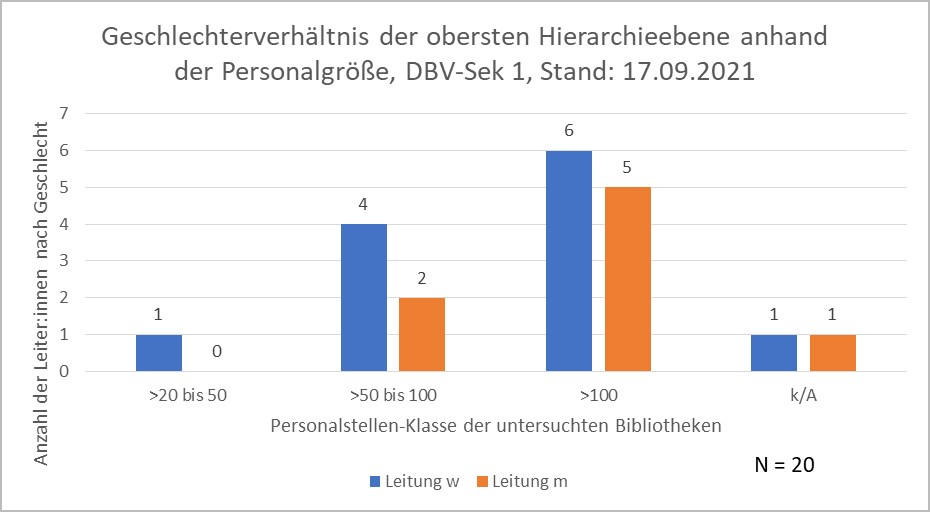
\includegraphics{img/Abb_01_DBV-Sek1.jpg}
\caption{Abbildung 1: Geschlechterverhältnis der Leitungsebene der
DBV-Sektion 1 anhand der Betriebsgröße}
\end{figure}

Die Auswertung (Abbildung 1) zeigt, dass der Anteil der Frauen zwar
insgesamt höher ist als jener der Männer, sich die Werte bei zunehmender
Bibliotheksgröße aber annähern.

In die Auswertung für Sektion 2 wurden 86 Bibliotheken einbezogen
(Abbildung 2). Die Einrichtungen mit \textgreater20 bis 50
Personalstellen sind am häufigsten in dieser Sektion vertreten. Der
Frauenanteil ist in diesem Bereich verhältnismäßig am größten und
entspricht ungefähr dem Gesamtanteil von Frauen im gesamten Berufsfeld.
Man sieht allerdings auch, dass das Verhältnis von Frauen und Männern in
den Bibliotheken mit über 50 Stellen annähernd ausgeglichen ist.

\begin{figure}
\centering
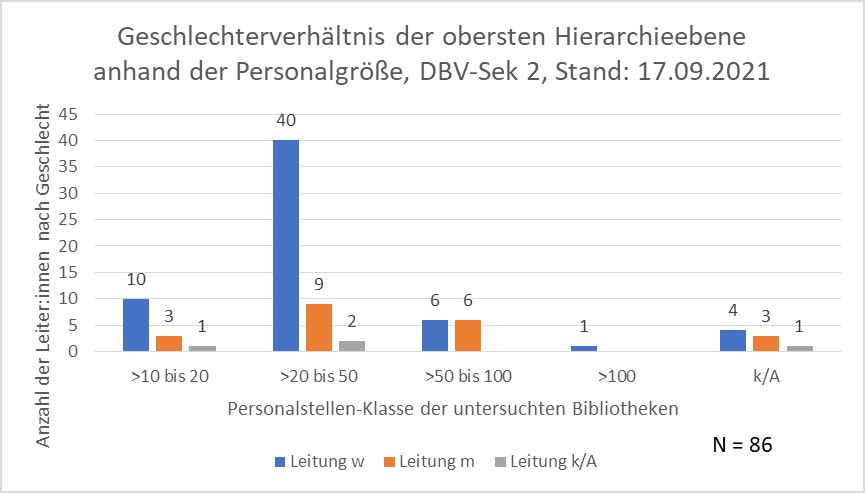
\includegraphics{img/Abb_02_DBV-Sek2.jpg}
\caption{Abbildung 2: Geschlechterverhältnis der Leitungsebene der
DBV-Sektion 2 anhand der Betriebsgröße}
\end{figure}

In Sektion 3A, in der zum Auszählungszeitpunkt 104 Einrichtungen
gelistet waren, finden sich, anhand der Personalstellen gemessen,
kleinere Bibliotheken im Vergleich zu den Sektionen 1 und 2 (Abbildung
3). Die Einrichtungen mit \textgreater10 bis 20 Personalstellen sind am
häufigsten in dieser Sektion vertreten und weisen auch einen merklich
höheren Anteil an Frauen in Leitungspositionen auf als Männer.

\begin{figure}
\centering
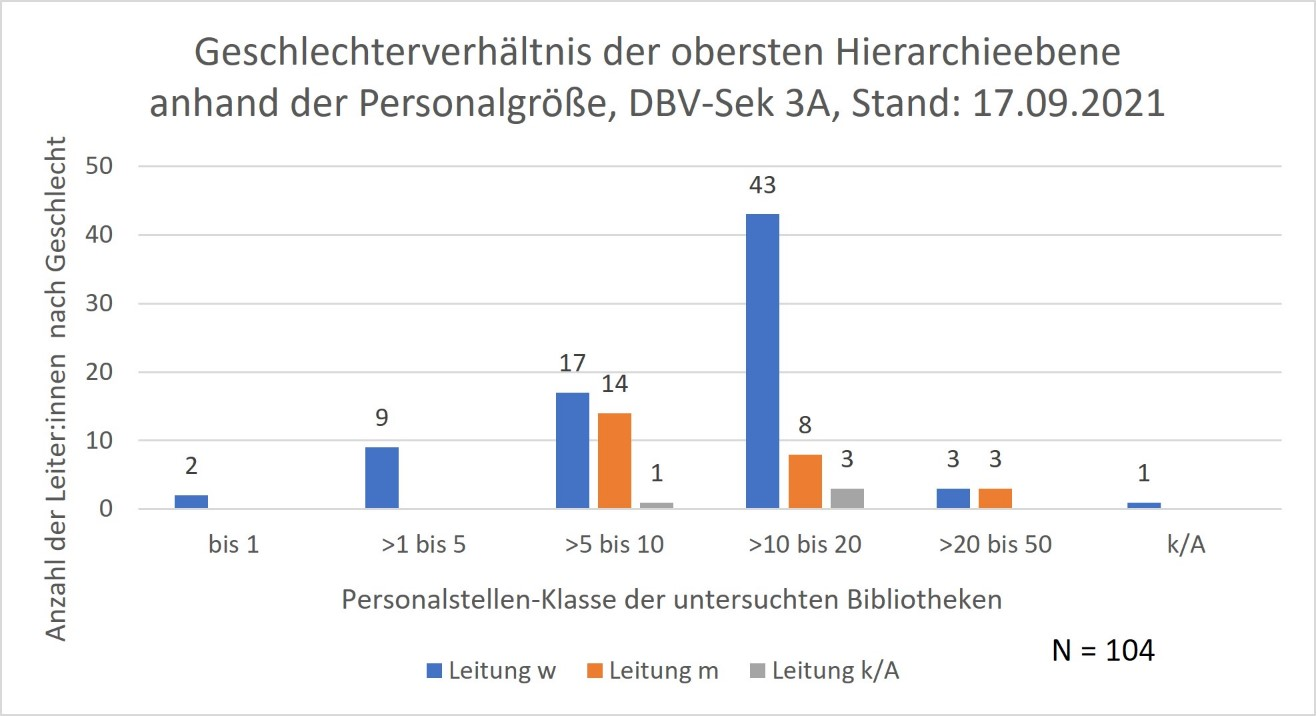
\includegraphics{img/Abb_03_DBV-Sek3A.jpg}
\caption{Abbildung 3: Geschlechterverhältnis der Leitungsebene der
DBV-Sektion 3A anhand der Betriebsgröße}
\end{figure}

Die Sektion 3B ist die zahlenmäßig größte Sektion unter den
DBV-Mitgliedern. Hier wurden Daten zu 1.169 Einrichtungen erhoben
(Abbildung 4). Die Einrichtungen mit \textgreater1 bis 5 Personalstellen
sind am häufigsten in dieser Sektion vertreten. Im Vergleich zu Männern
sind Frauen dort um das 8,5fache häufiger in der obersten
Hierarchieebene vertreten. Unter allen Sektionen ist Sektion 3B jene mit
dem geringsten Männeranteil.

\begin{figure}
\centering
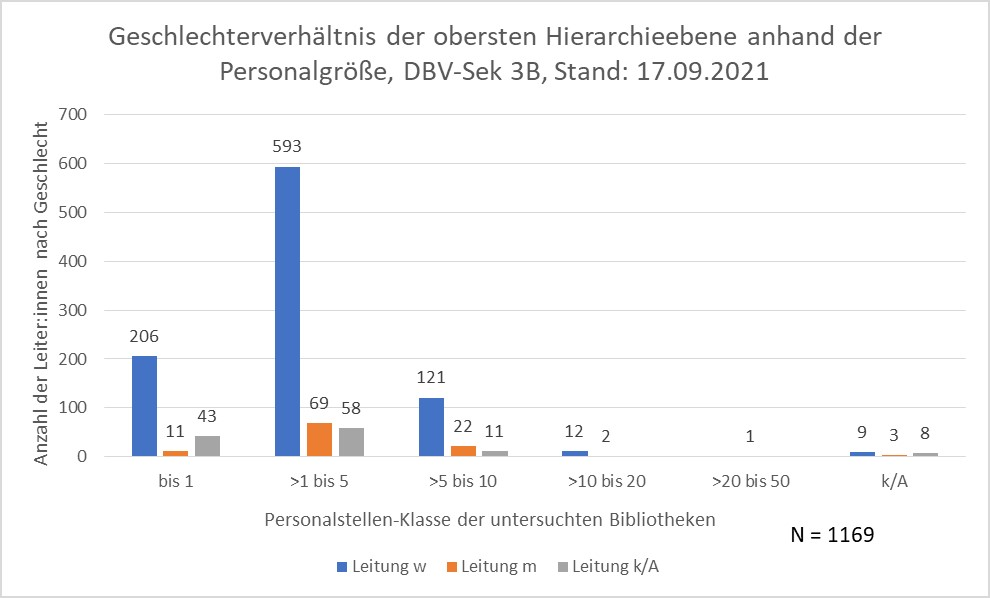
\includegraphics{img/Abb_04_DBV-Sek3B.jpg}
\caption{Abbildung 4: Geschlechterverhältnis der Leitungsebene der
DBV-Sektion 3B anhand der Betriebsgröße}
\end{figure}

Für die öffentlichen Bibliotheken lässt sich insgesamt festhalten, dass
der Anteil von Frauen in Leitungspositionen größer ist als der Anteil
der männlichen Leiter. Insbesondere bei kleineren Bibliotheken ist er
deutlich höher als jener der Männer. Mit zunehmender Bibliotheksgröße
nähern sich diese Werte an, wobei der Anteil der Männer mit einer
Ausnahme (Sektion 3B, \textgreater20 bis Personalstellen) nie höher ist
als der Frauenanteil.

Im Vergleich dazu ergibt sich für wissenschaftliche Bibliotheken ein
anderes Bild. Sektion 4 umfasst die wissenschaftlichen
Universalbibliotheken. Insgesamt wurden hierfür Daten von 292
Einrichtungen ausgewertet (Abbildung 5). Der Großteil dieser
Bibliotheken hat \textgreater1 bis 20 Personalstellen. Der Anteil der
Frauen in Leitungspositionen ist hier höher und insbesondere in
Bibliotheken mit \textgreater1 bis 5 Personalstellen signifikant größer.
Allerdings zeigt die Erhebung auch einen wesentlichen Unterschied zu den
Daten für die öffentlichen Bibliotheken. In Einrichtungen mit mehr als
20 Personalstellen ist der Anteil der Männer in Leitungspositionen
größer als jener der Frauen.\footnote{Für die Staatsbibliothek zu Berlin
  war in der DBV-Mitgliederliste noch eine Frau als Direktorin vermerkt.
  Zum Zeitpunkt der Auszählung war jedoch bereits ein männlicher
  Nachfolger eingesetzt. Dies wurde in der Erhebung berücksichtigt.}

\begin{figure}
\centering
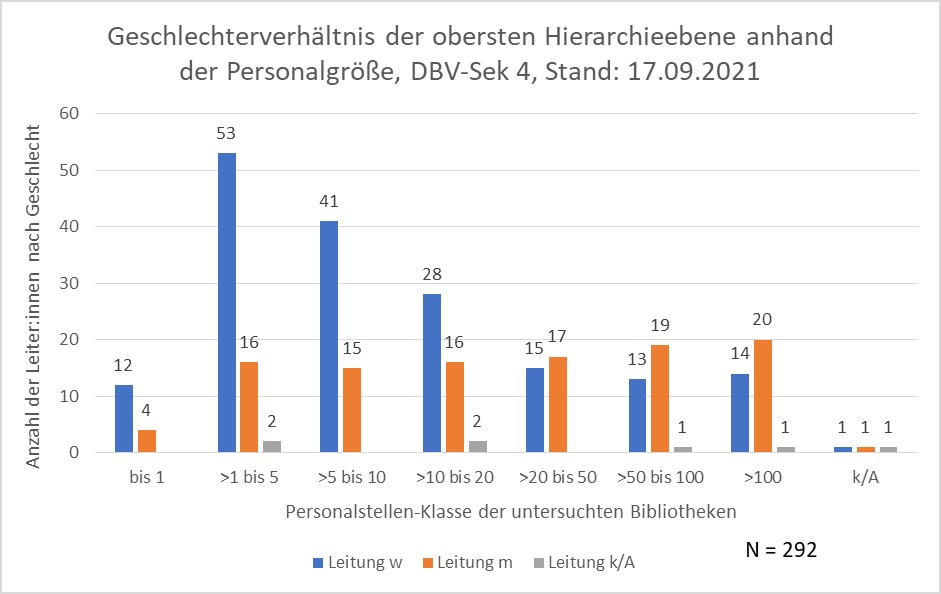
\includegraphics{img/Abb_05_DBV-Sek4.jpg}
\caption{Abbildung 5: Geschlechterverhältnis der Leitungsebene der
DBV-Sektion 4 anhand der Betriebsgröße}
\end{figure}

Die Mitglieder der Sektion 5 sind wissenschaftliche Spezialbibliotheken.
Von der Betriebsgröße lassen sich diese Einrichtungen mit denen aus
Sektion 3B aus dem ÖB-Bereich vergleichen. So haben von den 261
Bibliotheken der Sektion 5 nur acht Institutionen mehr als 20
Personalstellen (Abbildung 6). In Bibliotheken mit bis zu fünf
Personalstellen ist auch in diesem Fall der Frauenanteil um ein
Vielfaches höher als jener der Männer. Herauszustellen ist noch, dass in
Einrichtungen mit \textgreater{} 5 bis 10 Personalstellen mehr Männer in
Leitungspositionen zu finden sind als Frauen.

\begin{figure}
\centering
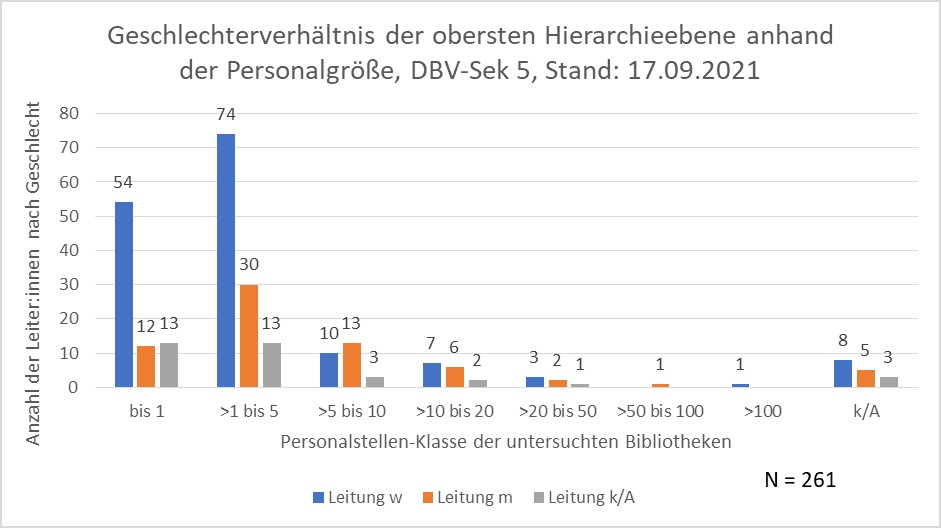
\includegraphics{img/Abb_06_DBV-Sek5.jpg}
\caption{Abbildung 6: Geschlechterverhältnis der Leitungsebene der
DBV-Sektion 5 anhand der Betriebsgröße}
\end{figure}

Um eine Entwicklung über die Jahre nachzeichnen zu können, werden im
Folgenden kurz die Auszählungen anhand der Betriebsgröße der Jahrbücher
der öffentlichen Bibliotheken (JÖB) sowie der Jahrbücher der Deutschen
Bibliotheken (VDB-Jahrbücher) vorgestellt.

\paragraph{5.2.1.2 Auswertung der Jahrbücher der öffentlichen Bibliotheken}

Die Erhebung in den JÖB erfolgte jeweils anhand von Fragebögen, die an
hauptamtlich geleitete öffentliche Bibliotheken in Deutschland
verschickt wurden. Gerade für die Jahrgänge 2002/03 und 2012/13 muss man
festhalten, dass ein wesentlicher Teil der verzeichneten Bibliotheken
keine Angabe zu Leitung und Personalgröße beinhalten. Die Auszählung der
Jahrbücher für diesen Beitrag ergibt ein ähnliches Bild für öffentliche
Bibliotheken wie die Auszählung der DBV-Mitgliederstatistik (Abbildungen
7--9). Insbesondere in Betrieben mit bis zu zehn Personalstellen ist der
Frauenanteil um ein Vielfaches höher als jener der Männer. Mit
zunehmender Bibliotheksgröße sinkt der Frauenanteil im Verhältnis.

\begin{figure}
\centering
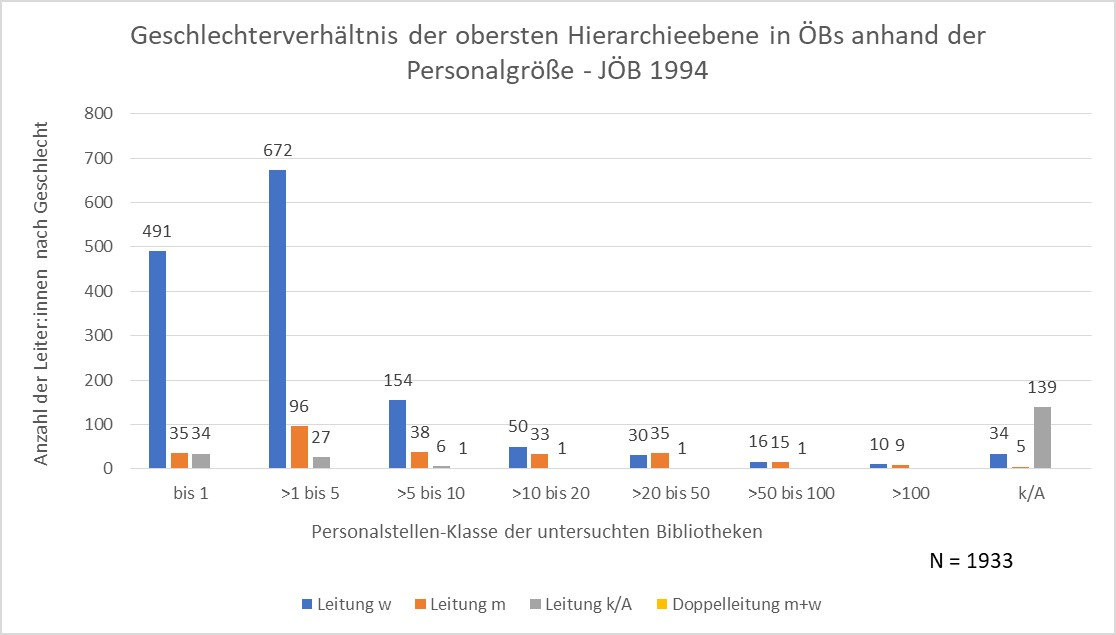
\includegraphics{img/Abb_07_JOB-1994.jpg}
\caption{Abbildung 7: Geschlechterverhältnis der Leitungsebene in
öffentlichen Bibliotheken anhand der Betriebsgröße, JÖB 1994}
\end{figure}

\begin{figure}
\centering
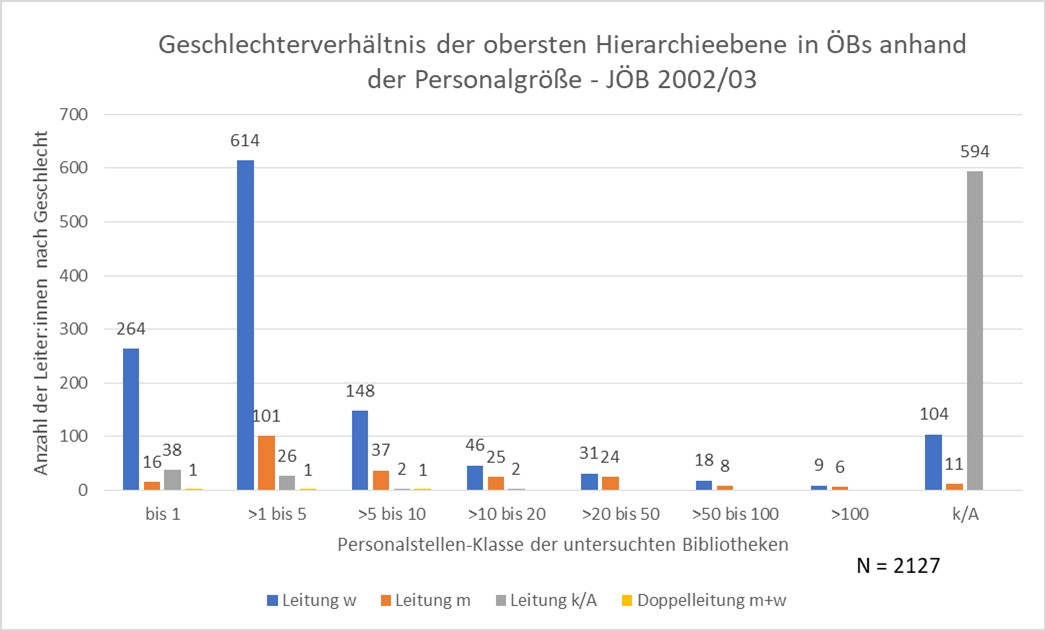
\includegraphics{img/Abb_08_JOB-2002.jpg}
\caption{Abbildung 8: Geschlechterverhältnis der Leitungsebene in
öffentlichen Bibliotheken anhand der Betriebsgröße, JÖB 2002/03}
\end{figure}

\begin{figure}
\centering
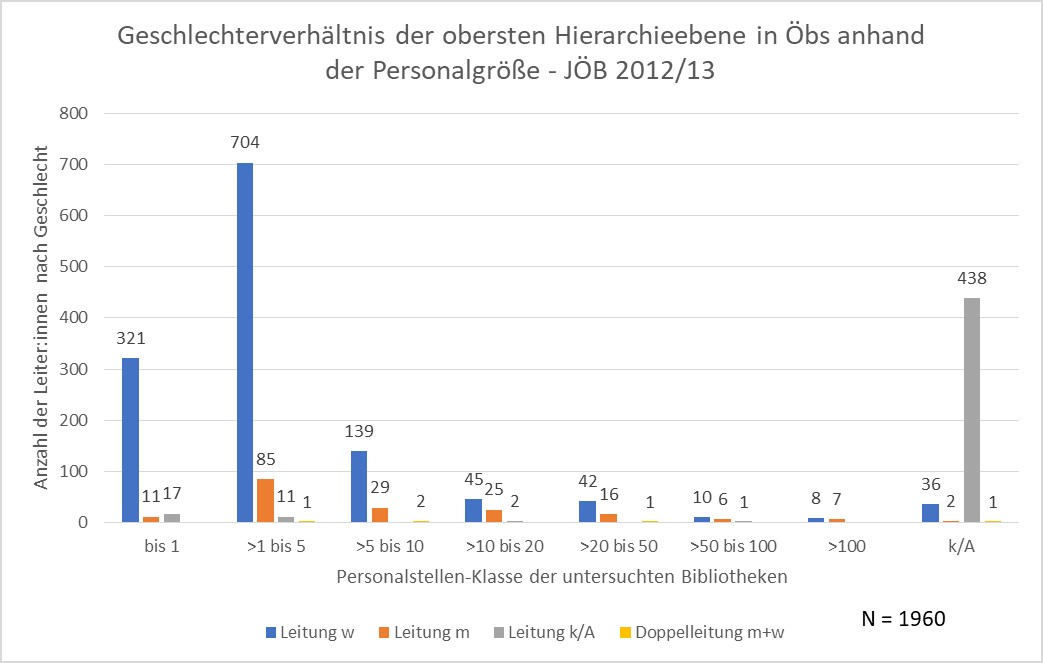
\includegraphics{img/Abb_09_JOB-2012.jpg}
\caption{Abbildung 9: Geschlechterverhältnis der Leitungsebene in
öffentlichen Bibliotheken anhand der Betriebsgröße, JÖB 2012/13}
\end{figure}

\paragraph{5.2.1.3 Auswertung der VDB-Jahrbücher}

Die Einträge in den VDB-Jahrbüchern beruhen auf Meldungen der
verzeichneten Bibliotheken. Die zeitliche Entwicklung zeigt, dass sich
der Frauenanteil in Leitungspositionen an wissenschaftlichen
Bibliotheken sukzessive erhöht hat. 1991 waren nur in Einrichtungen mit
bis zu fünf Personalstellen mehr Frauen als Männer in einer
Leitungsposition beschäftigt (Abbildung 10). In größeren Bibliotheken
überwog der Männeranteil, wobei der Frauenanteil mit Zunahme der
Betriebsgröße kontinuierlich abnahm. Für den Jahrgang 2001/02 kann man
bereits eine Verschiebung feststellen (Abbildung 11). Auch wenn der
Männeranteil noch überwiegt, sind hier auch in Bibliotheken mit
\textgreater10 bis 20 Personalstellen die Leitungspositionen nun
mehrheitlich von Frauen besetzt. 2011/12 ist das Verhältnis von Frauen
und Männern in Leitungspositionen nahezu ausgewogen (Abbildung 12).
Allerdings zeigt die Auswertung, dass Frauen vornehmlich in kleineren
Bibliotheken in Leitungspositionen sind. In Bibliotheken mit mehr als 20
Personalstellen findet sich eine umgekehrte Ausgangslage. Männer in
Leitungspositionen sind in diesen Einrichtungen häufiger vertreten als
Frauen.

\begin{figure}
\centering
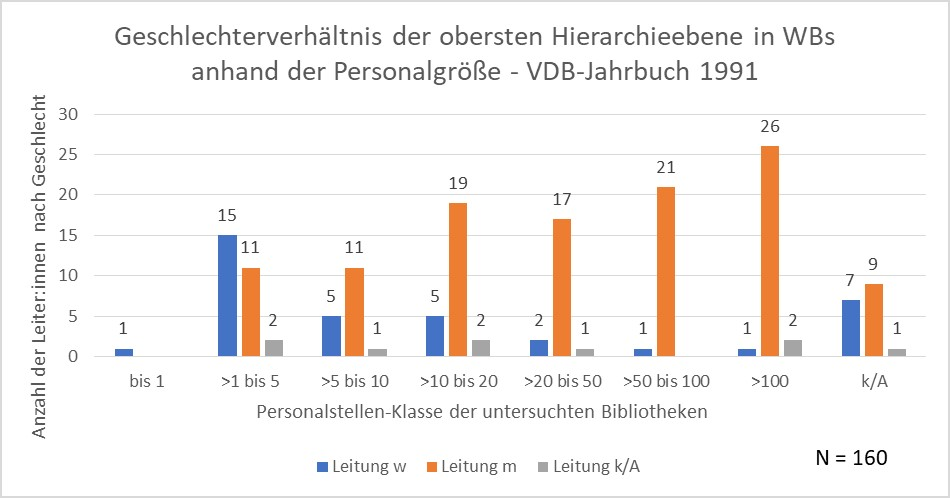
\includegraphics{img/Abb_10_VDB-1991.jpg}
\caption{Abbildung 10: Geschlechterverhältnis der Leitungsebene in
öffentlichen Bibliotheken anhand der Betriebsgröße, VDB-Jahrbuch 1991}
\end{figure}

\begin{figure}
\centering
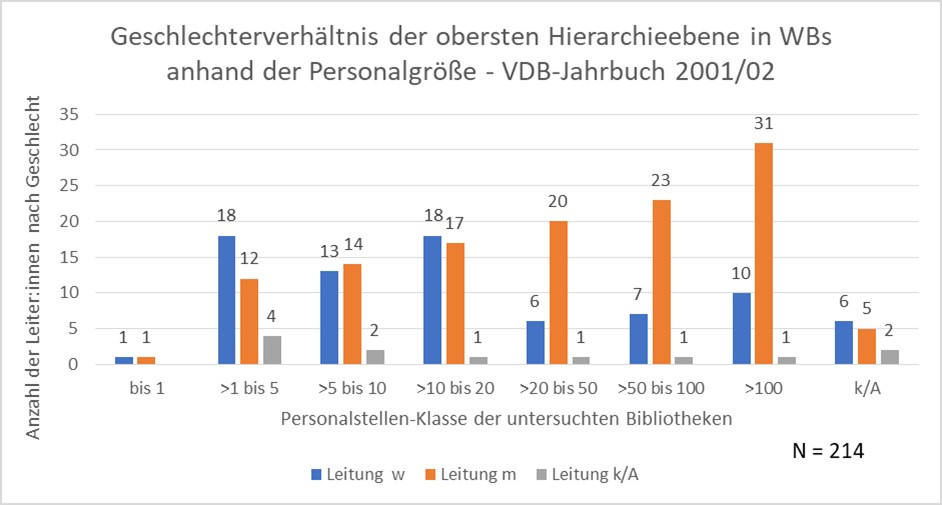
\includegraphics{img/Abb_11_VDB-2001.jpg}
\caption{Abbildung 11: Geschlechterverhältnis der Leitungsebene in
öffentlichen Bibliotheken anhand der Betriebsgröße, VDB-Jahrbuch
2001/02}
\end{figure}

\begin{figure}
\centering
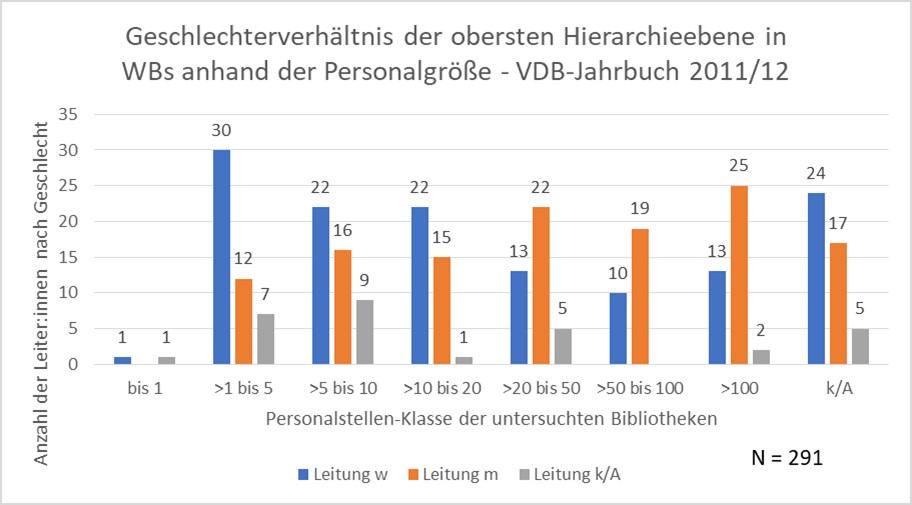
\includegraphics{img/Abb_12_VDB-2011.jpg}
\caption{Abbildung 12: Geschlechterverhältnis der Leitungsebene in
öffentlichen Bibliotheken anhand der Betriebsgröße, VDB-Jahrbuch
2011/12}
\end{figure}

\hypertarget{auswertung-in-gesamtzahlen}{%
\subsubsection{5.2.2 Auswertung in
Gesamtzahlen}\label{auswertung-in-gesamtzahlen}}

Nach der Verteilung von Frauen- und Männeranteilen in deutschen
Bibliotheken anhand der Einrichtungsgröße wurden die gesammelten Daten
in Gesamtzahlen nach Frauen- und Männeranteil ausgewertet, um die
vorausgegangenen Ausführungen überblicksartig zusammenzuführen. Da die
Verzeichnisse und Jahrbücher auf Angaben der verzeichneten Einrichtungen
beruhen und erwartungsgemäß nicht jede Institution, etwa aufgrund von
Zeit-/Personalmangel, Daten abliefert, hat sich in jeder Auszählung ein
gewisser Anteil an Bibliotheken ergeben, für den keine Informationen zu
der Leitung verfügbar ist. Insbesondere die JÖBs der Jahre 2002/03 und
2012/13 weisen einen sehr hohen Anteil an diesen Daten auf. Die
folgenden Darstellungen zeigen der Vollständigkeit halber daher zum
einen die Gesamtzahlen inklusive dieser unbekannten Variablen und zum
anderen eine \enquote{bereinigte} Version, in dem die Bibliotheken ohne
Angabe zur Leitung herausgerechnet wurden, auf die sich die folgenden
Ausführungen beziehen.

\paragraph{5.2.2.1 Auswertung der DBV-Mitgliederliste, Stand: 2021}

Die Auswertung der Gesamtzahlen zeigt für die öffentlichen Bibliotheken,
dass in allen Sektionen (1-3) die Mehrzahl der Leitungspositionen von
Frauen besetzt ist. Die durchschnittliche Bibliotheksgröße sinkt von
Sektion zu Sektion, sodass in Sektion 3B generell die kleinsten
Bibliotheken, gemessen anhand der Personalstellen, zu finden sind.
Betrachtet man die Verteilung des Frauenanteils auf diese Weise, so
stellt man fest, dass der Frauenanteil mit der Abnahme der
Bibliotheksgröße steigt. In den Bibliotheken der Sektion 1 liegt der
Anteil weiblicher Führungskräfte noch unterhalb dem Gesamtanteil der
weiblichen Beschäftigten (Abbildung 13). In den Sektionen 2 und 3A
stimmen die Werte annähernd überein (Abbildungen 15 und 17) und in
Sektion 3B liegt der Anteil weiblicher Führungskräfte sogar deutlich
über dem Gesamtdurchschnitt (Abbildung 19). Rechnet man die Werte aller
Sektionen zusammen, so ergibt sich zusammenfassend für die öffentlichen
Bibliotheken dennoch ein Anteil weiblicher Führungskräfte, der über dem
Prozentsatz weiblicher Mitarbeiterinnen im Allgemeinen liegt (Abbildung
21).

\begin{figure}
\centering
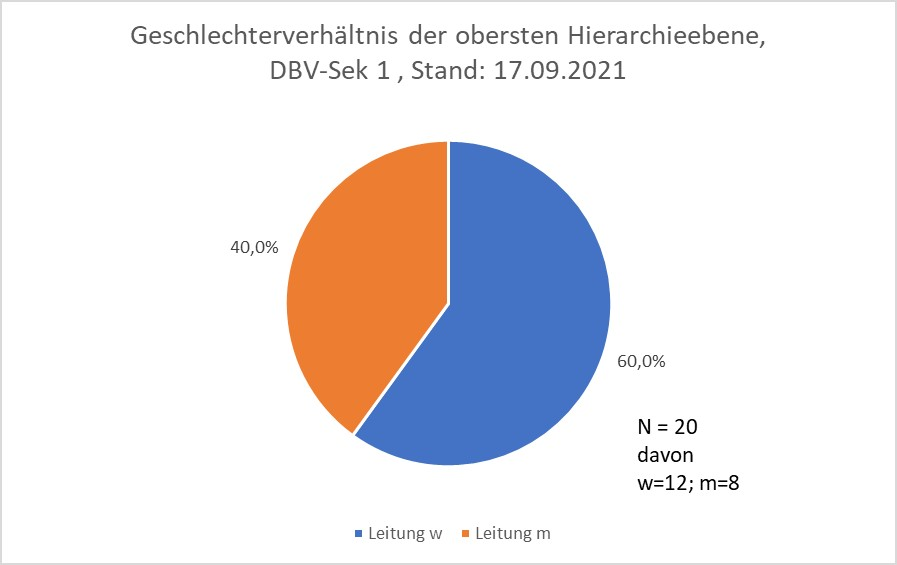
\includegraphics{img/Abb_13_DBV-Sek1_gesamt.jpg}
\caption{Abbildung 13: Geschlechterverhältnis in Gesamtzahlen für
DBV-Sektion 1}
\end{figure}

\begin{figure}
\centering
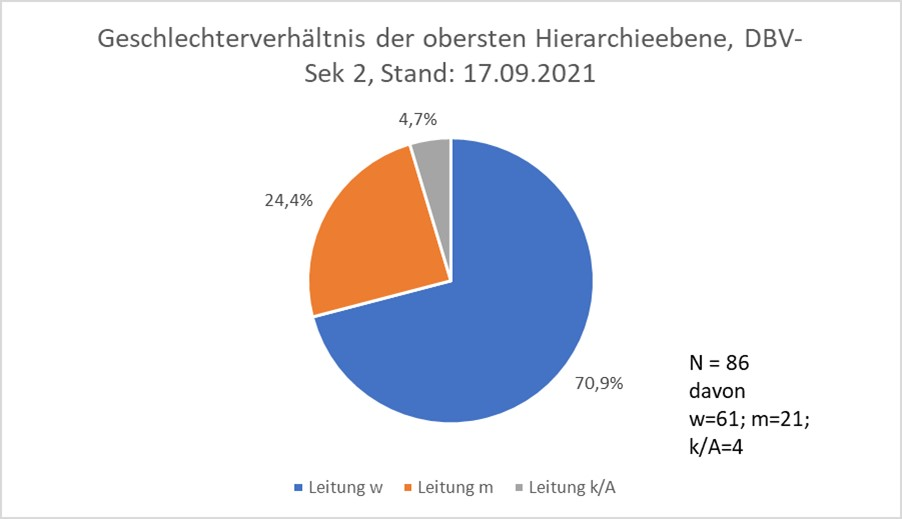
\includegraphics{img/Abb_14_DBV-Sek2_gesamt.jpg}
\caption{Abbildung 14: Geschlechterverhältnis in Gesamtzahlen für
DBV-Sektion 2}
\end{figure}

\begin{figure}
\centering
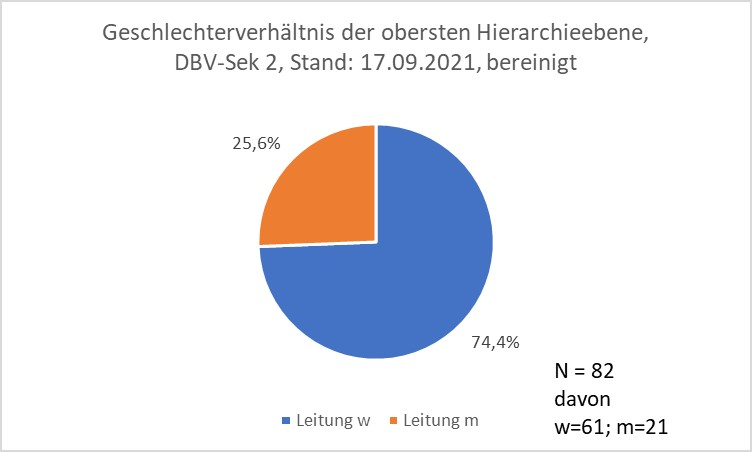
\includegraphics{img/Abb_15_DBV-Sek2_gesamt_bereinigt.jpg}
\caption{Abbildung 15: Geschlechterverhältnis in Gesamtzahlen für
DBV-Sektion 2, bereinigte Version}
\end{figure}

\begin{figure}
\centering
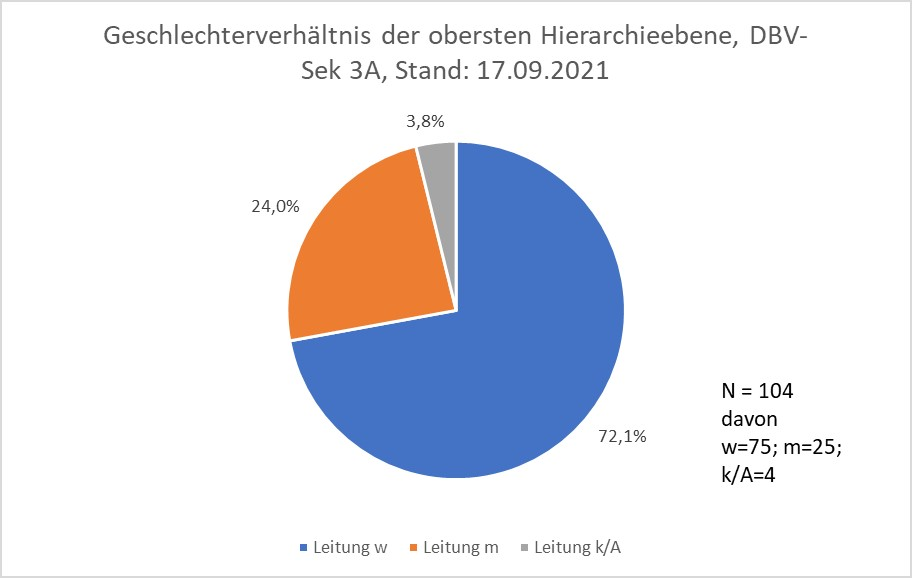
\includegraphics{img/Abb_16_DBV-Sek3A_gesamt.jpg}
\caption{Abbildung 16: Geschlechterverhältnis in Gesamtzahlen für
DBV-Sektion 3A}
\end{figure}

\begin{figure}
\centering
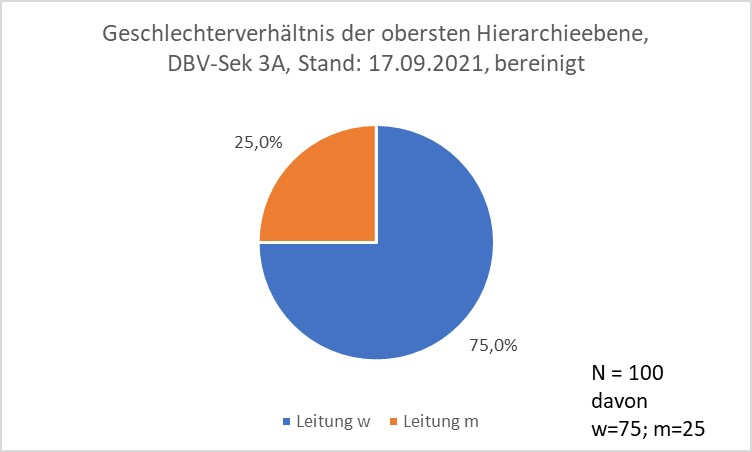
\includegraphics{img/Abb_17_DBV-Sek3A_gesamt_bereinigt.jpg}
\caption{Abbildung 17: Geschlechterverhältnis in Gesamtzahlen für
DBV-Sektion 3A, bereinigte Version}
\end{figure}

\begin{figure}
\centering
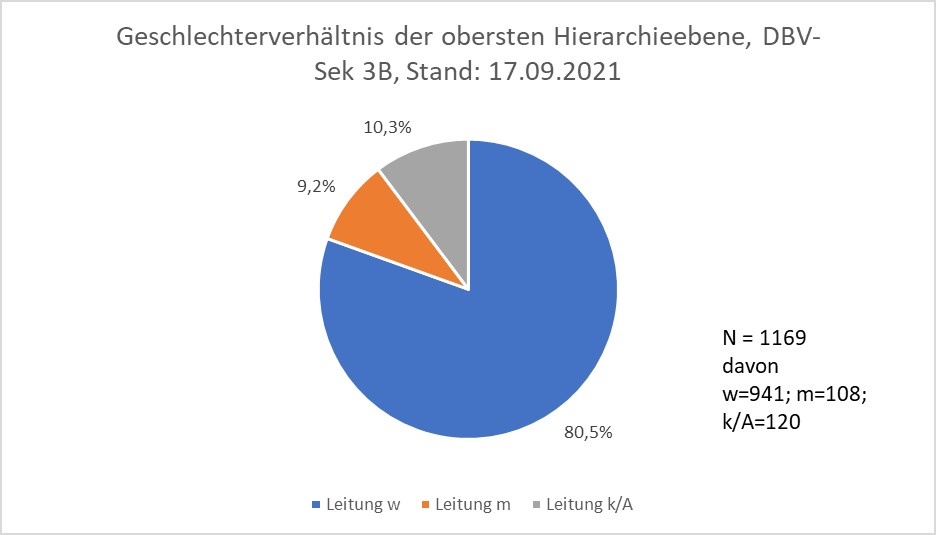
\includegraphics{img/Abb_18_DBV-Sek3B_gesamt.jpg}
\caption{Abbildung 18: Geschlechterverhältnis in Gesamtzahlen für
DBV-Sektion 3B}
\end{figure}

\begin{figure}
\centering
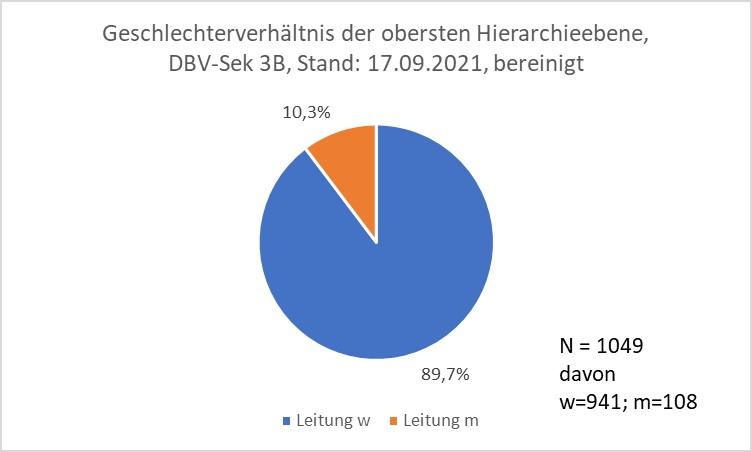
\includegraphics{img/Abb_19_DBV-Sek3B_gesamt_bereinigt.jpg}
\caption{Abbildung 19: Geschlechterverhältnis in Gesamtzahlen für
DBV-Sektion 3B, bereinigte Version}
\end{figure}

\begin{figure}
\centering
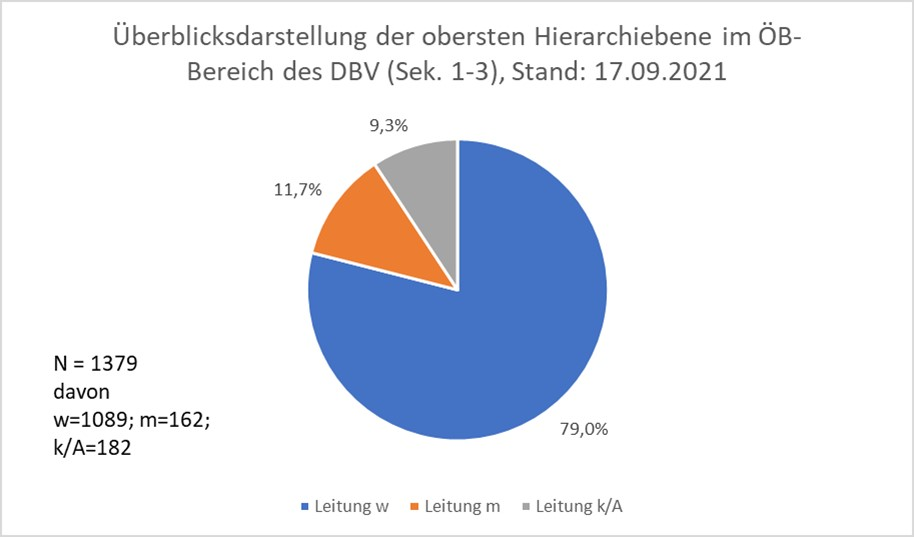
\includegraphics{img/Abb_20_DBV-Sek1-3_gesamt.jpg}
\caption{Abbildung 20: Geschlechterverhältnis in Gesamtzahlen für die
öffentlichen Bibliotheken (DBV-Mitglieder)}
\end{figure}

\begin{figure}
\centering
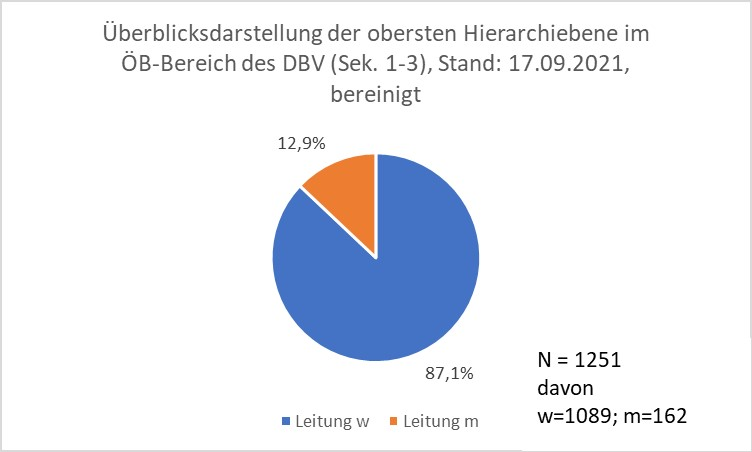
\includegraphics{img/Abb_21_DBV-Sek1-3_gesamt_bereinigt.jpg}
\caption{Abbildung 21: Geschlechterverhältnis in Gesamtzahlen für die
öffentlichen Bibliotheken (DBV-Mitglieder), bereinigte Version}
\end{figure}

\begin{figure}
\centering
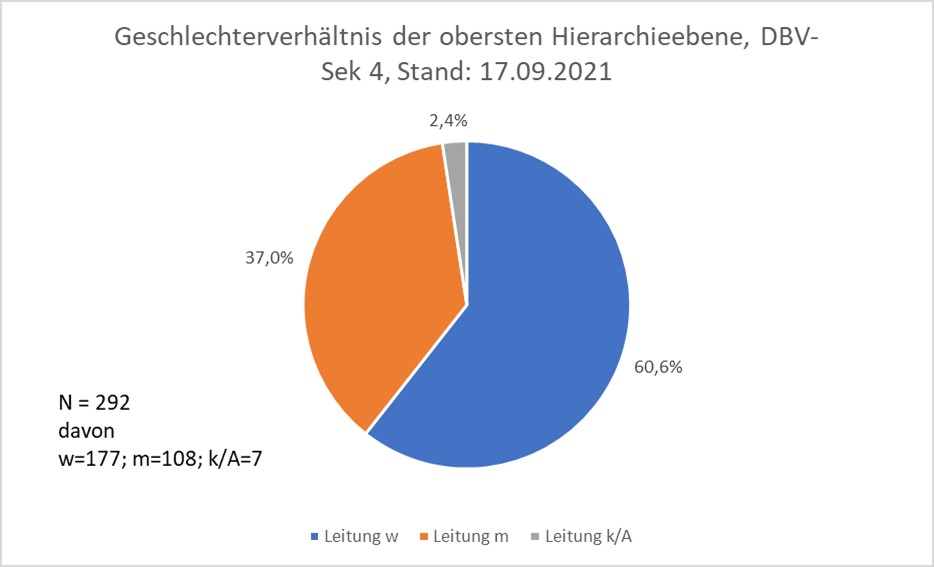
\includegraphics{img/Abb_22_DBV-Sek4_gesamt.jpg}
\caption{Abbildung 22: Geschlechterverhältnis in Gesamtzahlen für
DBV-Sektion 4}
\end{figure}

\begin{figure}
\centering
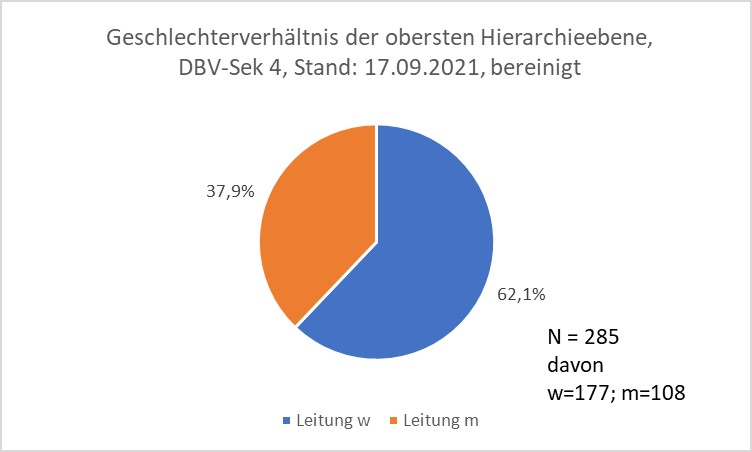
\includegraphics{img/Abb_23_DBV-Sek4_gesamt_bereinigt.jpg}
\caption{Abbildung 23: Geschlechterverhältnis in Gesamtzahlen für
DBV-Sektion 4, bereinigte Version}
\end{figure}

\begin{figure}
\centering
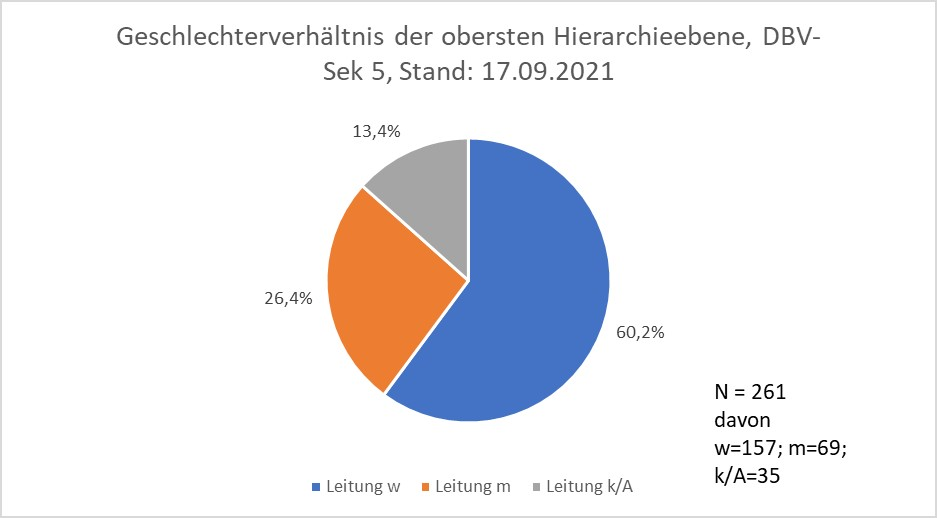
\includegraphics{img/Abb_24_DBV-Sek5_gesamt.jpg}
\caption{Abbildung 24: Geschlechterverhältnis in Gesamtzahlen für
DBV-Sektion 5}
\end{figure}

\begin{figure}
\centering
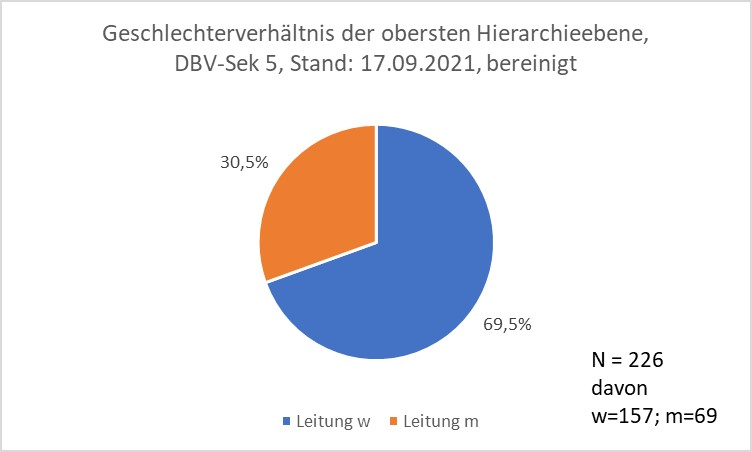
\includegraphics{img/Abb_25_DBV-Sek5_gesamt_bereinigt.jpg}
\caption{Abbildung 25: Geschlechterverhältnis in Gesamtzahlen für
DBV-Sektion 5, bereinigte Version}
\end{figure}

\begin{figure}
\centering
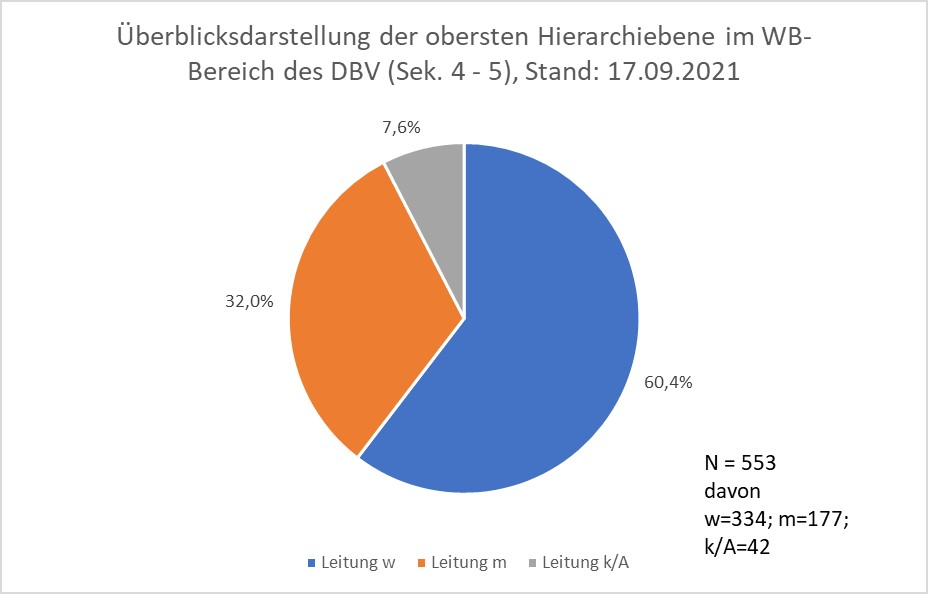
\includegraphics{img/Abb_26_DBV-Sek4-5_gesamt.jpg}
\caption{Abbildung 26: Geschlechterverhältnis in Gesamtzahlen für die
wissenschaftlichen Bibliotheken (DBV-Mitglieder}
\end{figure}

\begin{figure}
\centering
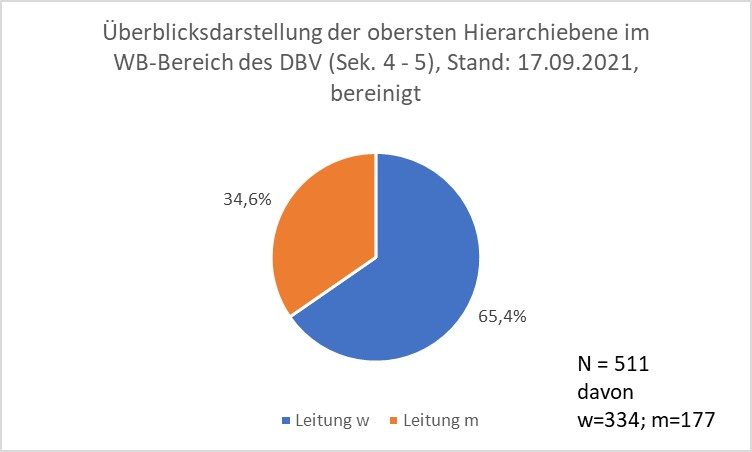
\includegraphics{img/Abb_27_DBV-Sek4-5_gesamt_bereinigt.jpg}
\caption{Abbildung 27: Geschlechterverhältnis in Gesamtzahlen für die
wissenschaftlichen Bibliotheken (DBV-Mitglieder), bereinigte Version}
\end{figure}

Die Auswertung der Gesamtzahlen zeigt für die wissenschaftlichen
Bibliotheken der DBV-Mit\-glied\-er\-liste ebenfalls, dass in den beiden
Sektionen 4 und 5 die Mehrzahl der Leitungspositionen von Frauen besetzt
ist (Abbildung 27). Allerdings ist die prozentuale Verteilung von
weiblicher zu männlicher Führungskraft nicht so deutlich wie in den
öffentlichen Bibliotheken. Denn sind dort nur etwa 12\% der
Führungskräfte männlich, liegt der Anteil der Männer in
Leitungspositionen für die wissenschaftlichen Bibliotheken bei etwa
einem Drittel.

\paragraph{5.2.2.2 Auswertung der Jahrbücher der öffentlichen Bibliotheken}

Wie eingangs dieses Unterkapitels bereits erläutert, gab es bei jeder
Quelle einen gewissen Prozentsatz in den Daten, der keine Angaben zur
Leitung der jeweiligen Einrichtung liefert. Insbesondere bei den beiden
jüngsten Jahrgängen des JÖB ist dieser Anteil mit über 20\%
beziehungsweise 30\% im Verhältnis zu den übrigen Jahrbüchern sehr hoch,
sodass sich in der Zeitreihe eine nicht nachvollziehbare Entwicklung des
Frauenanteils ergeben würde, von einem hohen Eingangswert mit über 75\%,
auf nur noch 58\% neun Jahre später. In den bereinigten Darstellungen
sind die Anteile konstant hoch und mit jeweils über 80\% höher als die
prozentuale Gesamtzahl weiblicher Beschäftigte in Bibliotheken
(Abbildungen 29, 31 und 33).

\begin{figure}
\centering
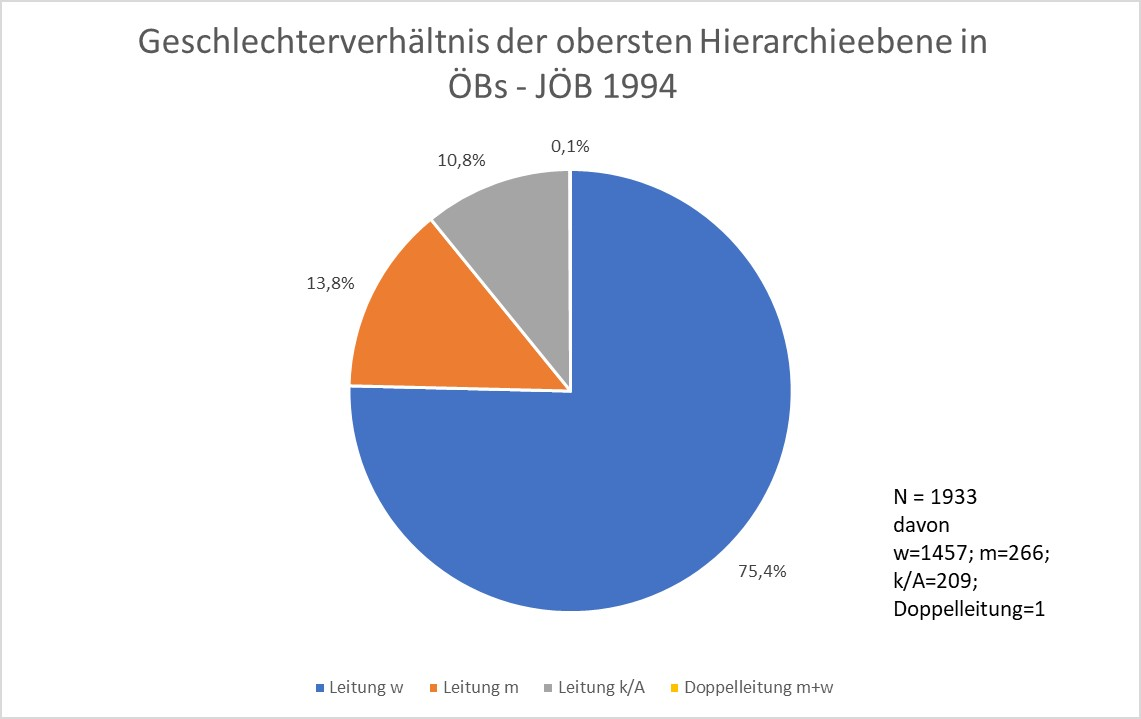
\includegraphics{img/Abb_28_JOB-1994_gesamt.jpg}
\caption{Abbildung 28: Geschlechterverhältnis in Gesamtzahlen für
öffentliche Bibliotheken, Auszählung JÖB 1994}
\end{figure}

\begin{figure}
\centering
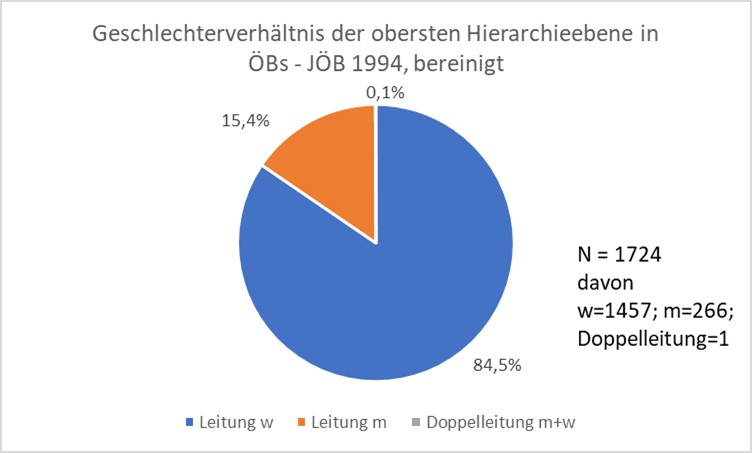
\includegraphics{img/Abb_29_JOB-1994_gesamt_bereinigt.jpg}
\caption{Abbildung 29: Geschlechterverhältnis in Gesamtzahlen für
öffentliche Bibliotheken, Auszählung JÖB 1994, bereinigte Version}
\end{figure}

\begin{figure}
\centering
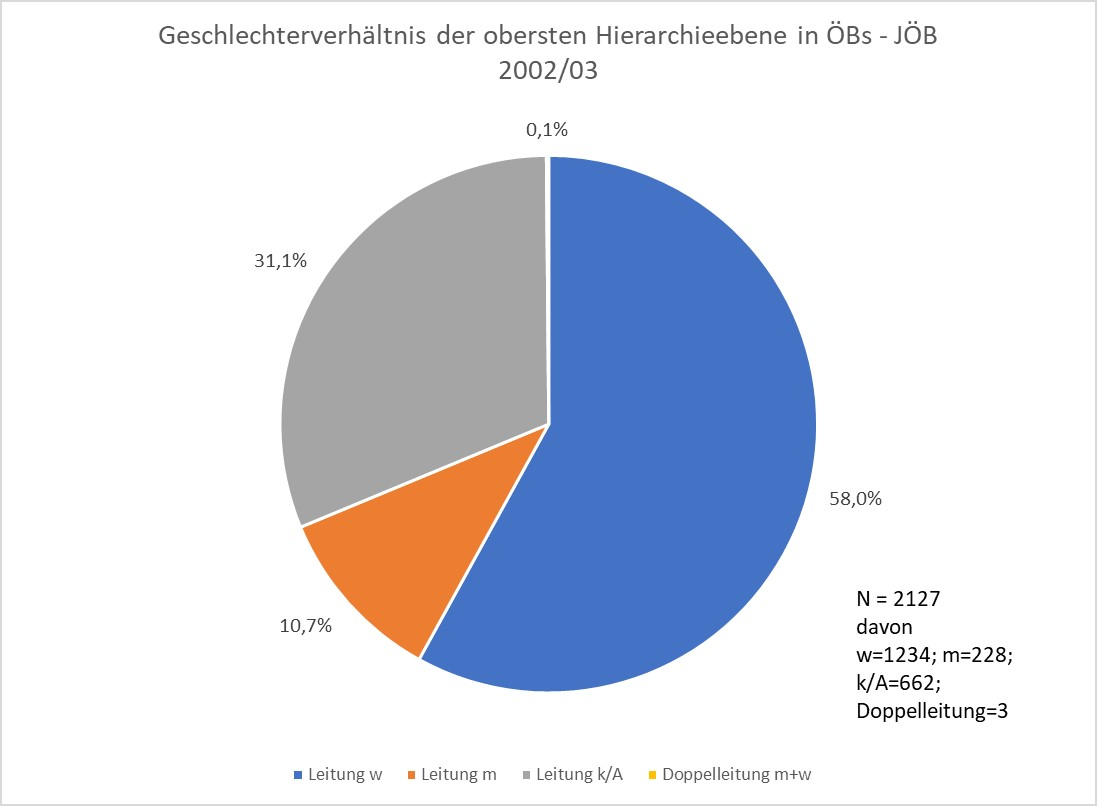
\includegraphics{img/Abb_30_JOB-2002_gesamt.jpg}
\caption{Abbildung 30: Geschlechterverhältnis in Gesamtzahlen für
öffentliche Bibliotheken, Auszählung JÖB 2002/03}
\end{figure}

\begin{figure}
\centering
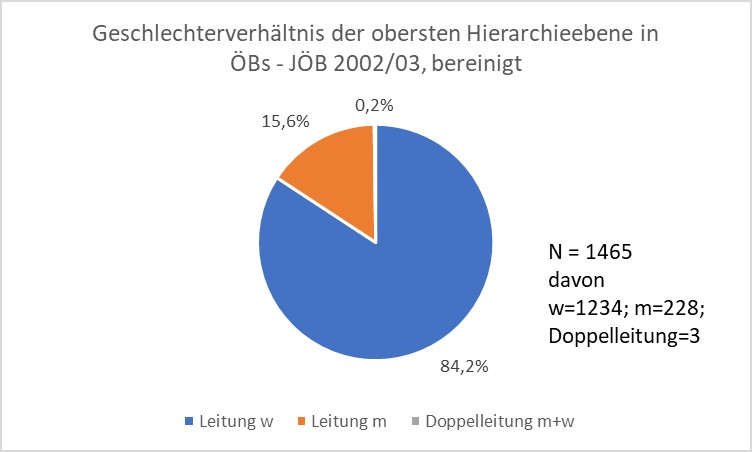
\includegraphics{img/Abb_31_JOB-2002_gesamt_bereinigt.jpg}
\caption{Abbildung 31: Geschlechterverhältnis in Gesamtzahlen für
öffentliche Bibliotheken, Auszählung JÖB 2002/03, bereinigte Version}
\end{figure}

\begin{figure}
\centering
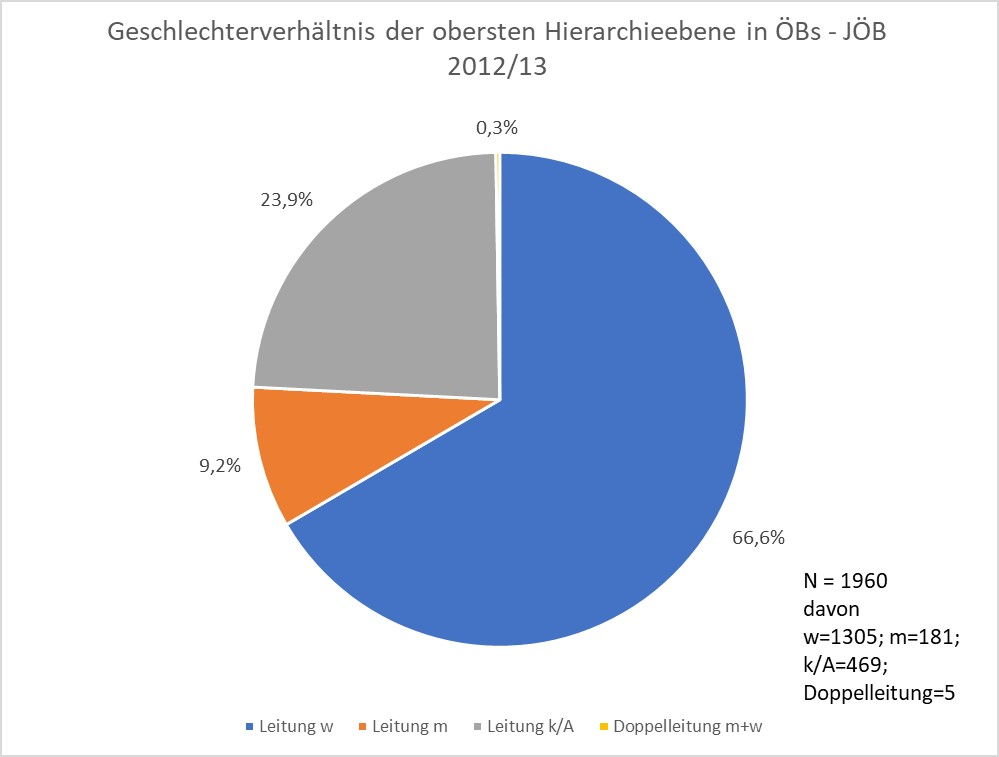
\includegraphics{img/Abb_32_JOB-2012_gesamt.jpg}
\caption{Abbildung 32: Geschlechterverhältnis in Gesamtzahlen für
öffentliche Bibliotheken, Auszählung JÖB 2012/13}
\end{figure}

\begin{figure}
\centering
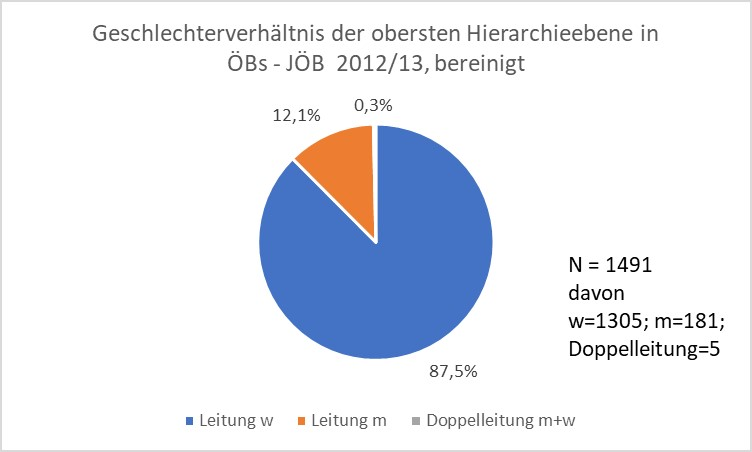
\includegraphics{img/Abb_33_JOB-2012_gesamt_bereinigt.jpg}
\caption{Abbildung 33: Geschlechterverhältnis in Gesamtzahlen für
öffentliche Bibliotheken, Auszählung JÖB 2012/13, bereinigte Version}
\end{figure}

\paragraph{5.2.2.3 Auswertung der VDB-Jahrbücher}

Für die Entwicklung der Geschlechterverteilung auf der Führungsebene an
wissenschaftlichen Bibliotheken ist über die Zeit eine dynamischere
Entwicklung zu beobachten. Für 2021 liegt der Anteil weiblicher
Führungskräfte bei über 65\% (bereinigte Version). Die Auszählung des
frühesten Jahrbuchs, das in die Erhebung mit aufgenommen wurde, ist für
das Jahr 1991. Dort ergeben sich nach der Auszählung noch umgekehrte
Vorzeichen. Der Anteil der männlichen Führungskräfte ist mit drei
Vierteln der Gesamtanzahl an ausgezählten Daten so hoch wie zu keinem
anderen Zeitpunkt (Abbildung 35). In den Folgejahren nimmt der Anteil
der Frauen stetig zu (Abbildung 37) und die Daten aus 2011/12 zeigen
erstmals für den gesamten WB-Bereich einen höheren Anteil an weiblichen
als an männlichen Führungskräften (Abbildung 39).

\begin{figure}
\centering
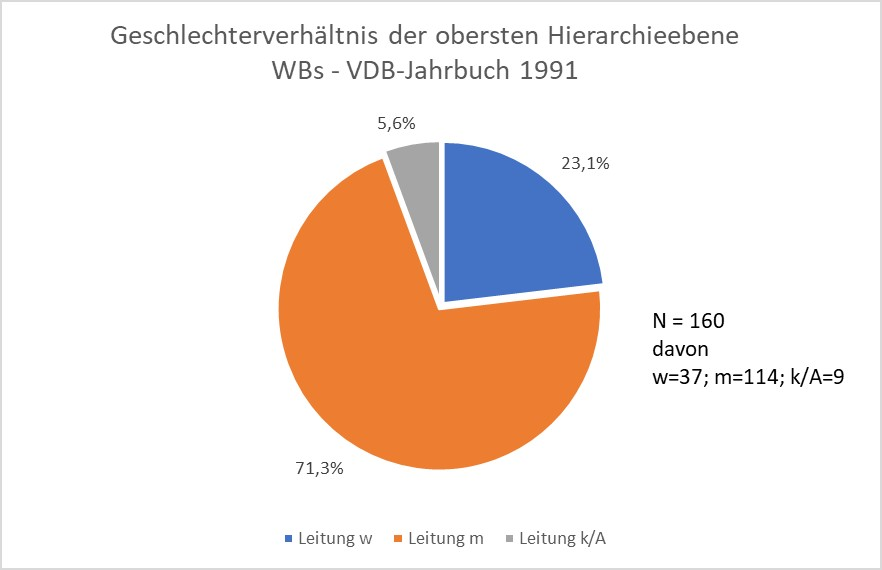
\includegraphics{img/Abb_34_VDB-1991_gesamt.jpg}
\caption{Abbildung 34: Geschlechterverhältnis in Gesamtzahlen für
wissenschaftliche Bibliotheken, Auszählung VDB-Jahrbuch 1991}
\end{figure}

\begin{figure}
\centering
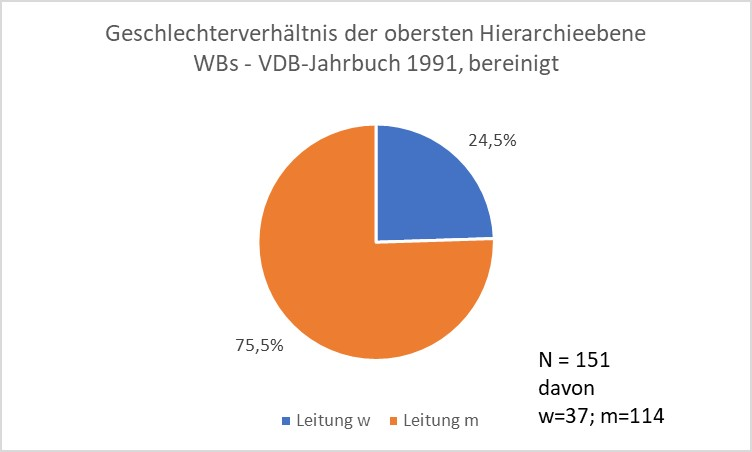
\includegraphics{img/Abb_35_VDB-1991_gesamt_bereinigt.jpg}
\caption{Abbildung 35: Geschlechterverhältnis in Gesamtzahlen für
wissenschaftliche Bibliotheken, Auszählung VDB-Jahrbuch 1991, bereinigte
Version}
\end{figure}

\begin{figure}
\centering
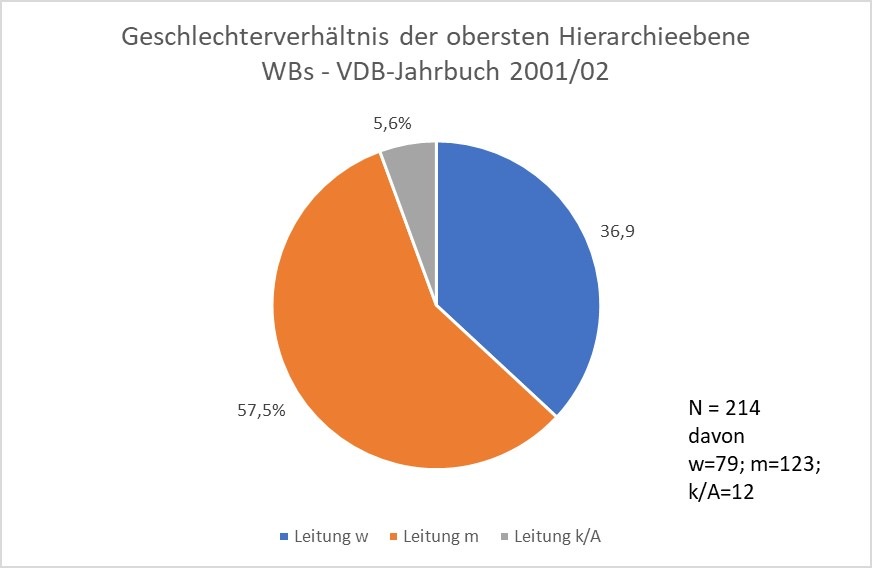
\includegraphics{img/Abb_36_VDB-2001_gesamt.jpg}
\caption{Abbildung 36: Geschlechterverhältnis in Gesamtzahlen für
wissenschaftliche Bibliotheken, Auszählung VDB-Jahrbuch 2001/02}
\end{figure}

\begin{figure}
\centering
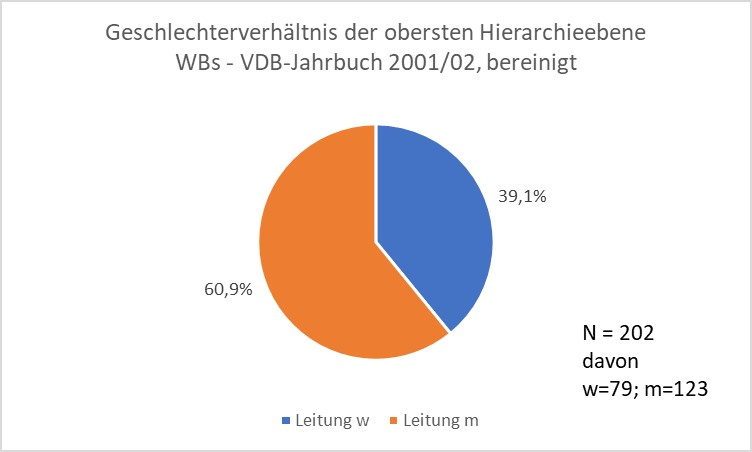
\includegraphics{img/Abb_37_VDB-2001_gesamt_bereinigt.jpg}
\caption{Abbildung 37: Geschlechterverhältnis in Gesamtzahlen für
wissenschaftliche Bibliotheken, Auszählung VDB-Jahrbuch 2001/02,
bereinigte Version}
\end{figure}

\begin{figure}
\centering
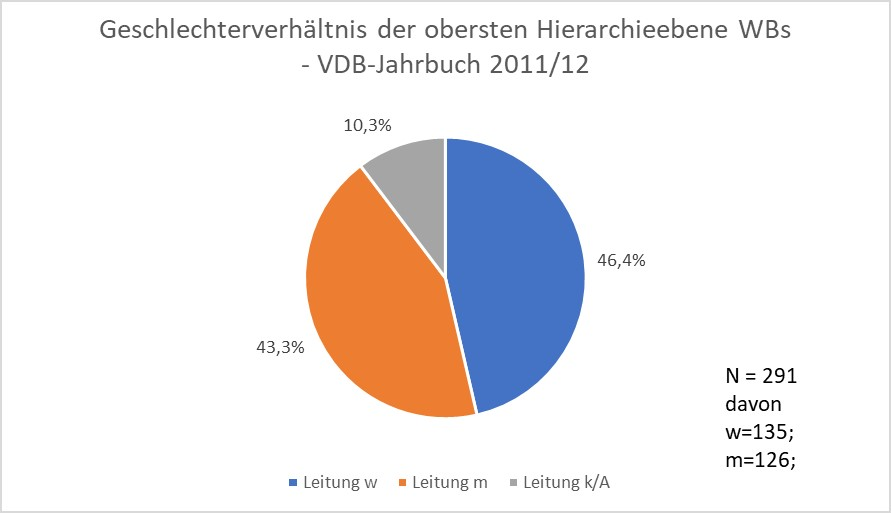
\includegraphics{img/Abb_38_VDB-2011_gesamt.jpg}
\caption{Abbildung 38: Geschlechterverhältnis in Gesamtzahlen für
wissenschaftliche Bibliotheken, Auszählung VDB-Jahrbuch 2011/12}
\end{figure}

\begin{figure}
\centering
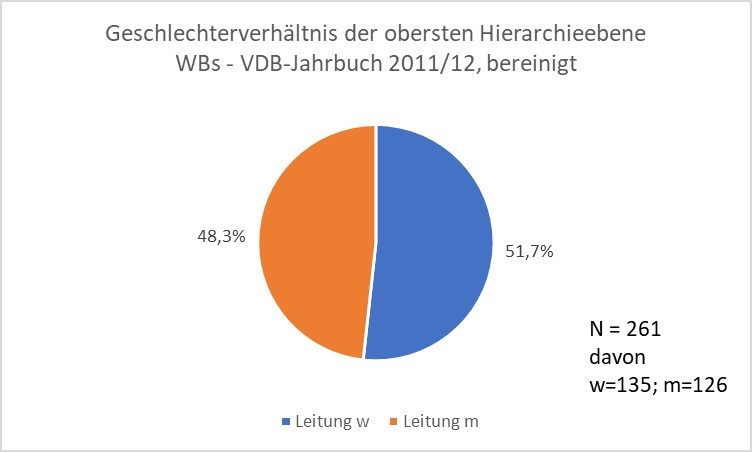
\includegraphics{img/Abb_39_VDB-2011_gesamt_bereinigt.jpg}
\caption{Abbildung 39: Geschlechterverhältnis in Gesamtzahlen für
wissenschaftliche Bibliotheken, Auszählung VDB-Jahrbuch 2011/12,
bereinigte Version}
\end{figure}

\hypertarget{diskussion}{%
\section{6. Diskussion}\label{diskussion}}

Das Ziel der vorliegenden Untersuchung war die Schaffung einer
umfassenden Datenauswertung zu den aktuellen statistischen Verteilungen
von Frauen in Führungspositionen an deutschen Bibliotheken. Der
Überblick bereits vorhandener Untersuchungen in Kapitel 4 hat gezeigt,
dass die jüngsten aufbereiteten Daten bereits aus dem Jahr 2014 stammen.
Zudem ist der Fokus der meisten Studien entweder ausschnitthaft gewählt
oder die Ergebnisse sind nicht nachnutzbar.

Die umfassende Auswertung der verfügbaren Quellen schließt somit,
zumindest teilweise, eine bestehende Lücke im
bibliothekswissenschaftlichen Diskurs und sollte idealerweise als
Ausgangspunkt für weitere Diskussionen dienen.

Für die Arbeit erfolgte eine quantitative Erhebung anhand der
Mitgliederliste des deutschen Bibliotheksverbands (DBV) für den
aktuellen Zeitraum sowie ausgewählter Jahrbücher der deutschen
Bibliotheken und der öffentlichen Bibliotheken für frühere Jahrgänge, um
die Entwicklung der letzten 20--30 Jahre sichtbar machen zu können.

Bewusst wurde bei der Erhebung die Unterscheidung zwischen öffentlichen
und wissenschaftlichen Bibliotheken beibehalten. Die historische
Entwicklung des Berufsfeldes, das in Kapitel 2 dargelegt wurde, konnte
zeigen, dass sich die Etablierung von Frauen in den beiden Sparten
unterschiedlich schnell entwickelt hat. In der Tat zeigen die
Gesamtzahlen in der bereinigten Darstellung der hier vorliegenden
Datenauswertung, dass der Anteil von Frauen auf der obersten
Hierarchieebene in öffentlichen Bibliotheken in allen untersuchten
Jahren bei einem nahezu konstant hohen Wert von über 80\% liegt und
deutlich größer ist als bei wissenschaftlichen Bibliotheken (Abbildung
41). Für wissenschaftliche Bibliotheken zeigt sich über die Jahre eine
deutliche Entwicklung in den Geschlechterverhältnissen (Abbildung 43).
Lag der Frauenanteil auf der obersten Hierarchieebene 1991 noch bei
knapp unter 25\%, zeigt die Auswertung für 2021 einen Wert von 65,4\%.
Allerdings liegt dieser damit noch deutlich unter dem Gesamtanteil von
Frauen im Berufsfeld, was darauf hindeutet, dass öffentliche
Bibliotheken in der Tat bessere Aufstiegsmöglichkeiten für Frauen
bieten. So sind Frauen nach wie vor auf der Führungsebene von WBs
unterrepräsentiert, auch wenn die aktuellen Zahlen und die dargelegte
Entwicklung vermuten lassen, dass sich der Anteil weiter erhöhen wird.
Dies zeigt jedoch auch, dass unterschiedliche Richtungen eines
Berufsfeldes in unterschiedlichem Maße segregiert sein können.
Vergleicht man Sektion 3B (ÖB-Bereich) und Sektion 5 (WB), die sich in
der Verteilung der Personalstellen-Klassen ähneln, zeigt sich in der
bereinigten Version eine deutliche Diskrepanz in der Verteilung. Während
in Sektion 3B 89,7\% der obersten Leitungspositionen von Frauen besetzt
sind, liegt der Anteil in Sektion 5 bei 69,5\%.

Allgemeine Untersuchungen der Arbeitsmarktforschung zeigen, dass Frauen
in kleineren Betrieben leichter aufsteigen können als in großen
Betrieben. Die aktuelle Auszählung kann dies insbesondere für
wissenschaftliche Bibliotheken bestätigen. Auch wenn der Gesamtanteil
der Frauen in Leitungspositionen in Bibliotheken im Vergleich zu anderen
Berufsfeldern erfreulich hoch ist, ergeben sich doch auffällige Punkte,
die weiterführender Untersuchungen bedürfen.

Für öffentliche Bibliotheken zeigt die Erhebung, dass sich die
Verteilung von Männern und Frauen bei zunehmender Bibliotheksgröße
annähern, wobei der Anteil der Frauen immer noch höher ist als jener der
Männer. Für wissenschaftliche Bibliotheken ergibt sich ein anderes Bild.
Ab einer Bibliotheksgröße mit mehr als 20 Personalstellen ist der Anteil
in Leitungsposition höher als jener der Frauen. Prozesse, wie der in
Kapitel 3 beschriebene \enquote{glass escalator}-Effekt, könnten hier
greifen.

Die vorliegende Arbeit bietet eine umfassende Übersicht über die Anteile
von Frauen auf der obersten Hierarchieebene. Die Erfassung der
Verteilung der darunter gegliederten Segmente war durch die Methodenwahl
nicht möglich. In einem nächsten Schritt wäre die Untersuchung dieser
wünschenswert, um einen Überblick der dortigen Verteilung zu erhalten.

Abschließend lässt sich resümieren, dass die Entwicklung des Anteils von
Frauen auf der obersten Hierarchiestufe in wissenschaftlichen
Bibliotheken positiv verläuft und sich über die letzten 30 Jahre
kontinuierlich erhöht hat. Allerdings liegt er noch immer deutlich unter
jenem für öffentliche Bibliotheken, der über den gesamten
Untersuchungszeitraum konstant hoch war und sogar über dem Gesamtanteil
von Frauen in dem Berufsfeld liegt. Zudem konnte gezeigt werden, dass
Frauen insbesondere in kleineren Bibliotheken die Leitungsposition
innehaben. Die Ergebnisse dieser Studie liefern also eine umfassende
statistische Aufarbeitung der Geschlechterverhältnisse für die
Leitungspositionen an deutschen Bibliotheken, was der zugrundeliegenden
Leitfrage entspricht. Eine umfassend angelegte qualitative Studie könnte
offene Fragen nach potenziellen Gründen beleuchten. Generell ist also in
der weiteren Diskussion die Frage zu stellen, ob Frauen sich signifikant
häufiger für die Tätigkeit in öffentlichen Bibliotheken entscheiden oder
ob die Barrieren für Frauen in wissenschaftlichen Bibliotheken
aufzusteigen, tatsächlich höher sind, da die Diskrepanz in der
Verteilung der beiden Sparten anhand der statistischen Zahlen merklich
ist. Für eine gleichstellungsbezogene Durchmischung müsste die
prozentuale Verteilung der Bibliotheksleiter:innen dem Gesamtanteil des
jeweiligen Geschlechts im Berufsfeld entsprechen. Der Anteil von 65,4\%
(bereinigte Version) für wissenschaftliche Bibliotheken liegt somit
immer noch knapp zehn Prozentpunkte unterhalb des Gesamtanteils an
Frauen im Bibliotheksbereich. In den Arbeiten von Laura Stadler (STADLER
2012) sowie Birte Gerber, Bianca Mundt und Ines Rabe (GERBER/MUNDT/RABE
2005) klingen bereits kritische zu hinterfragende Punkte wie die
Vereinbarkeit von Familie und Beruf an.

\begin{figure}
\centering
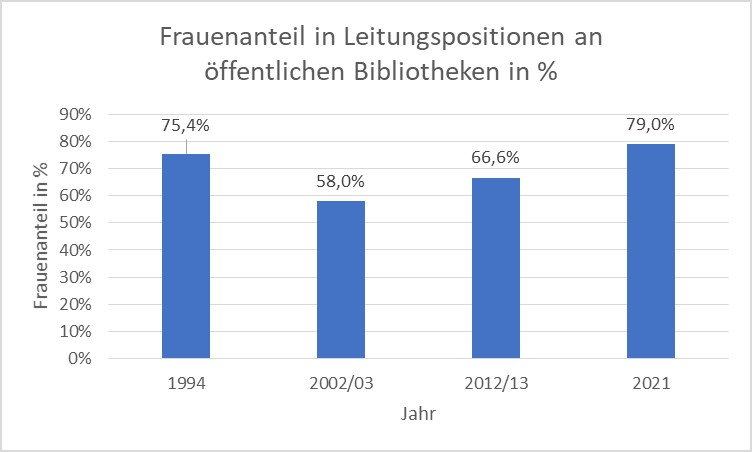
\includegraphics{img/Abb_40_Zeitreihe-OB.jpg}
\caption{Abbildung 40: Zeitreihe \enquote{Frauenanteil in
Leitungspositionen an öffentlichen Bibliotheken}}
\end{figure}

\begin{figure}
\centering
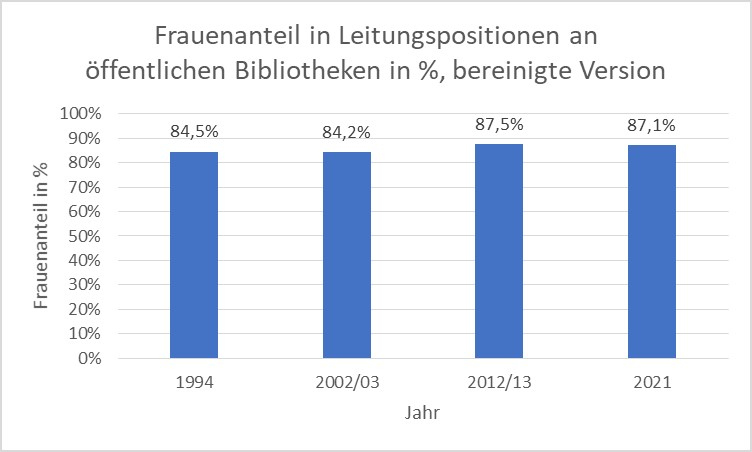
\includegraphics{img/Abb_41_Zeitreihe-OB_bereinigt.jpg}
\caption{Abbildung 41: Zeitreihe \enquote{Frauenanteil in
Leitungspositionen an öffentlichen Bibliotheken}, bereinigte Version}
\end{figure}

\begin{figure}
\centering
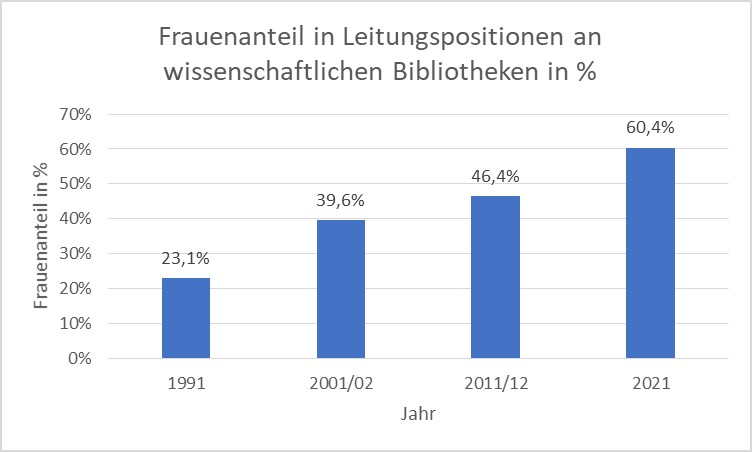
\includegraphics{img/Abb_42_Zeitreihe-WB.jpg}
\caption{Abbildung 42: Zeitreihe \enquote{Frauenanteil in
Leitungspositionen an wissenschaftlichen Bibliotheken}}
\end{figure}

\begin{figure}
\centering
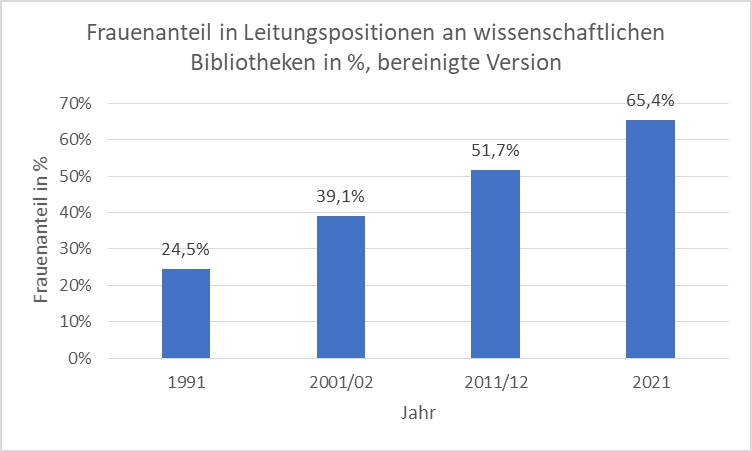
\includegraphics{img/Abb_43_Zeitreihe-WB_bereinigt.jpg}
\caption{Abbildung 43: Zeitreihe \enquote{Frauenanteil in
Leitungspositionen an wissenschaftlichen Bibliotheken}, bereinigte
Version}
\end{figure}

\hypertarget{danksagung}{%
\section{7. Danksagung}\label{danksagung}}

Ich danke Frau Dr.~Ulla Wimmer für ihre Unterstützung während des
gesamten Prozesses der Masterarbeit. Weiterhin gilt mein Dank den
Kolleg:innen des DBV für die Zusendung der Daten als Excel-Liste zur
abschließenden Prüfung der Erhebung.

\hypertarget{literaturverzeichnis}{%
\section{8. Literaturverzeichnis}\label{literaturverzeichnis}}

ACHATZ 2018: Achatz, Juliane (2018): Berufliche Geschlechtersegregation.
In: Abraham, Martin; Hinz, Thomas (Hg.): Arbeitsmarktsoziologie.
Probleme, Theorien, empirische Befunde. 3., überarbeitete und erweiterte
Auflage. Wiesbaden: Springer VS, S. 389--435.

BIBLIOTHEKEN 1993: Bundesvereinigung Deutscher Bibliotheksverbände
(1994): Bibliotheken '93: Strukturen - Aufgaben - Positionen. Berlin:
Deutsches Bibliotheksinstitut.

BIBLIOTHEKSPLAN 1973: Deutsche Bibliothekskonferenz (1973):
Bibliotheksplan 73. Entwurf eines umfassenden Bibliotheksnetzes für die
Bundesrepublik Deutschland. Berlin: Deutscher Büchereiverband,
Arbeitsstelle für das Büchereiwesen.

BMFSFJ 2021: Bundesministerium für Familie, Senioren, Frauen und Jugend:
Zweites Führungs-positionen-Gesetz - FüPoG II. Stand: 12.08.2021. URL:
\url{https://www.bmfsfj.de/bmfsfj/service/gesetze/zweites-fuehrungspositionengesetz-fuepog-2-164226}
(letzter Zugriff am 14.05.2023).

BUSCH 2013: Busch, Anne (2013): Die berufliche Geschlechtersegregation
in Deutschland. Ursachen, Reproduktion, Folgen. Wiesbaden: Springer VS.

BUSCH-HEIZMANN 2015: Busch-Heizmann, Anne (2015): Frauenberufe,
Männerberufe und die \enquote{Drehtür} -- Ausmaß und Implikationen für
West- und Ostdeutschland. In: WSI-Mitteilungen. 2015 (8), S. 571 -- 582.
URL: \url{https://www.wsi.de/data/wsimit_2015_08_busch-heizmann.pdf}
(letzter Zugriff am14.05.2023).

DBS 2021: URL:
\url{https://service-wiki.hbz-nrw.de/pages/viewpage.action?pageId=78577673}

(letzter Zugriff am 14.05.2023).

DESTATIS: Statistisches Bundesamt (Destatis): Teilhabe von Frauen am
Erwerbsleben. Stand: 2019. URL:
\url{https://www.destatis.de/DE/Themen/Arbeit/Arbeitsmarkt/Qualitaet-Arbeit/Dimension-1/teilhabe-frauen-erwerbsleben.html}
(letzter Zugriff am 14.05.2023).

GERBER/MUNDT/RABE 2005: Gerber, Birte; Mundt, Bianca; Rabe, Ines (2005):
Vergleich der Position bzw. Rolle der Frau in Öffentlichen Bibliotheken,
Wissenschaftlichen Bibliotheken und Informationseinrichtungen.
Auswertung einer Befragung. In: Krauss-Leichert, Ute: Interkulturelles
Online-Lernen. Die Rolle der Frau in Bibliotheken und
Informationseinrichtungen. Münster: Lit-Verlag, S. 61-96.

HACKER 2002: Hacker, Gerhard (2002): \enquote{Deine Zauber binden
wieder...} - Zur Überwindung der Spartentrennung in der Bibliotheks- und
Informationswissenschaft: Öffentliche Antrittsvorlesung anlässlich der
Berufung zum Professor, gehalten am 8. Mai 2002 am Fachbereich Buch und
Museum der HTWK Leipzig. Leipzig. URL:
\url{https://fim.htwk-leipzig.de/fileadmin/portal/f_m/Fakultaet_Medien/Personen/Professoren/07091.pdf}
(letzter Zugriff am 14.05.2023).

HAUSCHKE 2013: Hauschke, Christian (2013): Frauen in Führungspositionen
bei DBV-Mitgliedern. Stand: 18.03.2013. URL:
\url{https://infobib.de/2013/03/18/frauen-in-fuhrungspositionen-bei-dbv-mitgliedern/}
(letzter Zugriff am 14.05.2023).

HAUSMANN/KLEINERT 2014: Hausmann, Ann-Christin; Kleinert, Corinna
(2014): Berufliche Segregation auf dem Arbeitsmarkt. Männer- und
Frauendomänen kaum verändert. In: IAB-Kurzbericht. 2014 (9), S. 2--8.
URL: \url{https://doku.iab.de/kurzber/2014/kb0914.pdf} (letzter Zugriff
am 14.05.2023).

HEIDTMANN 1974: Heidtmann, Frank (1974): Die bibliothekarische
Berufswahl. Eine empirische Untersuchung der Berufswahl des
Bibliothekars des gehobenen Dienstes an öffentlichen und
wissenschaftlichen Bibliotheken. Pullach: Verl. Dokumentation
(Veröffentlichungen des Instituts für Bibliothekarausbildung der Freien
Universität Berlin, 3).

HENN 2009: Henn, Monika (2009): Die Kunst des Aufstiegs. Was Frauen in
Führungspositionen kennzeichnet. 2. Auflage. Frankfurt, New York:
Campus.

HINZ/GARTNER 2005: Hinz, Thomas; Gartner, Hermann (2005):
Geschlechtsspezifische Lohnunterschiede in Branchen, Berufen und
Betrieben / The Gender Wage Gap within Economic Sectors, Occupations,
and Firms. In: Zeitschrift für Soziologie 34 (1), S. 22-39. DOI:
\url{https://doi.org/10.1515/zfsoz-2005-0102} (letzter Zugriff
am14.05.2023).

IAB 2021: Institut für Arbeitsmarkt- und Berufsforschung: Berufe im
Spiegel der Statistik. URL:
\url{http://bisds.iab.de/Default.aspx?beruf=BG733\&region=1\&qualifikation=0}
(letzter Zugriff am 14.05.2023).

JANK 2000: Jank, Dagmar (2000): Frauen im Höheren Bibliotheksdienst vor
dem Zweiten Weltkrieg. In: Plassmann, Engelbert; Syré, Ludger (Hg.):
Verein Deutscher Bibliothekare 1900 - 2000. Festschrift. Wiesbaden:
Harrassowitz, S. 302--313.

KANTER 1977: Kanter, Rosabeth Moss (1977): Men and women of the
corporation. New York, NY: Basic Books.

KIRKLAND 1997: Kirkland, Janice J. (1997): The Missing Women Library
Directors: Deprivation versus Mentoring. In: CRL (College \& Research
Libraries) 58 (4), S. 375--383. DOI:
\url{https://doi.org/10.5860/crl.58.4.375} (letzter Zugriff am
14.05.2023).

KOHAUT/MÖLLER 2017: Kohaut, Susanne; Möller, Iris (2017):
Führungspositionen in Betrieben und Verwaltungen: Oberste Chefetage
bleibt Männerdomäne. Nürnberg (IAB-Kurzbericht, 24/2017). URL:
\url{http://doku.iab.de/kurzber/2019/kb2319.pdf} (letzter Zugriff am
14.05.2023).

KOHAUT/MÖLLER 2019: Kohaut, Susanne; Möller, Iris (2019): Frauen in
leitenden Positionen: Leider nichts Neues auf den Führungsetagen.
Nürnberg (IAB-Kurzbericht, 23/2019). URL:
\url{http://doku.iab.de/kurzber/2019/kb2319.pdf} (letzter Zugriff am
14.05.2023).

MORAN ET AL. 2009: Moran, Barbara B.; Leonard, Elisabeth; Zellers,
Jessica (2009): Women administ-rators in academic libraries: Three
decades of change. Library Trends, Vol. 58 (Nr. 2), S. 215-228. DOI:
\url{http://doi.org/10.1353/lib.0.0088} (letzter Zugriff am 14.05.2023).

OHLENDIECK 2003: Ohlendieck, Lutz (2003): Die Anatomie des Glashauses:
Ein Beitrag zum Verständnis des Glass-Ceiling-Phänomens. In: Pasero,
Ursula (Hg.): Gender - from Costs to Benefits. Wiesbaden: Westdt. Verl.,
S. 183--193.

PASSERA 2000: Passera, Carmen (2000): Frauen im wissenschaftlichen
Bibliotheksdienst nach 1945. In: Plassmann, Engelbert; Syré, Ludger
(Hg.): Verein Deutscher Bibliothekare 1900 - 2000. Festschrift.
Wiesbaden: Harrassowitz, S. 314--324.

PAWLOWSKI-FLODELL 1995: Pawlowski-Flodell, Charlotte (Hg.) (1995):
Berufsbild und Selbstverständnis der Bibliothekare in Deutschland 1994.
Erarbeitet von einer Arbeitsgruppe Berliner Bibliothekare. Berlin:
Deutsches Bibliotheksinstitut (dbi-materialien).

SCHELLE-WOLFF 2014: Schelle-Wolff, Carola: Mit dem Master in die
Bibliothek. In: BuB -- Forum Bibliothek und Information 66. Jg. 2018
(6), S. 450-453.

SCHILLER 1974: Schiller, Anita (1974): Women in Librarianship. In:
Advances in Librarianship, 1974 (4), S. 103--147.

SCHULZ ET AL. 2016: Schulz, Gabriele; Ries, Carolin; Zimmermann, Olaf
(2016): Frauen in Kultur und Medien. Ein Überblick über aktuelle
Tendenzen, Entwicklungen und Lösungsvorschläge. Berlin: Deutscher
Kulturrat.

STADLER 2012: Stadler, Laura (2012): Die Gläserne Decke in Schweizer
Bibliotheken. Chur: Schweizerisches Institut für
Informationswissenschaft, HTW Chur (Churer Schriften zur
Informationswissenschaft 53). URL:
\url{https://www.fhgr.ch/fileadmin/fhgr/angewandte_zukunftstechnologien/SII/churer_schriften/sii-churer_schriften_53-Glaeserne_Decke_in_Schweizer_Bibliotheken.pdf}
(letzter Zugriff am14.05.2023).

VODOSEK 1981: Vodosek, Peter (1981): Zur Entwicklung des
bibliothekarischen Berufs als Frauenberuf. In: BIBLIOTHEK Forschung und
Praxis 5 (3), S. 231--244.

\textbf{8. Quellen}

DBV SEKTIONEN 2021: Deutscher Bibliotheksverband e.V.: Sektionen --
Übersicht. Stand: 17.09.2021,

URL: \url{https://www.bibliotheksverband.de/fachgruppen/sektionen.html}
(letzter Zugriff am 14.05.2023).

JÖB 1994: Berufsverband Information Bibliothek e.V. (Hg.) (1994):
Jahrbuch der öffentlichen Bibliotheken, 1994. Bad Honnef: Bock +
Herchen.

JÖB 2002/03: Berufsverband Information Bibliothek e.V. (Hg.) (2002/03):
Jahrbuch der öffentlichen Bibliotheken, 2002/03. Bad Honnef: Bock +
Herchen.

JÖB 2012/13: Berufsverband Information Bibliothek e.V. (Hg.) (2012/13):
Jahrbuch der öffentlichen Bibliotheken, 2012/13. Bad Honnef: Bock +
Herchen.

VDB 1991: Verein Deutscher Bibliothekarinnen und Bibliothekare (1991):
Jahrbuch der Deutschen Bibliotheken 54, 1991. Wiesbaden: Harrassowitz.

VDB 2001/02: Verein Deutscher Bibliothekarinnen und Bibliothekare
(2001/02): Jahrbuch der Deutschen Bibliotheken 59, 2001/02. Wiesbaden:
Harrassowitz.

VDB 2011/12: Verein Deutscher Bibliothekarinnen und Bibliothekare
(2011/12): Jahrbuch der Deutschen Bibliotheken 64, 2011/12. Wiesbaden:
Harrassowitz.

%autor
\begin{center}\rule{0.5\linewidth}{0.5pt}\end{center}

\textbf{Julia Bartlewski} (\url{https://orcid.org/0000-0001-5959-4999})
hat Bibliotheks- und Informationswissenschaft (MA LIS) an der
Humboldt-Universität zu Berlin studiert und ist seit 2022 als
wissenschaftliche Mitarbeiterin an der Universitätsbibliothek Bielefeld
tätig.

\end{document}
